\documentclass[11pt]{article} 

\usepackage{graphicx}
\usepackage{subcaption}

    
%%% colores personalizados 
	\usepackage{xcolor}
		\definecolor{RojoNebrija}{RGB}{194,0,47}
		\definecolor{GrisNebrija1}{RGB}{127,127,127}
		\definecolor{GrisNebrija2}{RGB}{166,166,166}
		\definecolor{GrisNebrija3}{RGB}{191,191,191}
		
		
%%% traduce elementos al castellano, eg "figura" en lugar de "figure"
	\usepackage[spanish]{babel} 
	
	
%%% extractos de codigo
	\usepackage{minted}
%		\usemintedstyle{autumn}
		%\usemintedstyle{autumn}
        \usemintedstyle{manni}
        %\usemintedstyle{trac}
		
		
%%% Margenes
	\usepackage[a4paper, margin=2cm]{geometry}
	\addtolength{\topmargin}{-0.4cm}
	
%%% 1,5 espacios de interlineado
	\renewcommand{\baselinestretch}{1.5} 


%%%\renewcommand{\cftsecleader}{\cftdotfill{\cftdotsep}} % subsecciones en tabla de contenido
	\setcounter{tocdepth}{2}


%%% cambia el color y estilo de las secciones
	\usepackage{titlesec}
		\titleformat{\section} %a rojo y subrallado
			{\color{RojoNebrija}\normalfont\Large\bfseries}
			{\thesection}{1em}{}[{\titlerule[0.5pt]}]

		\titleformat{\subsubsection} % a gris, sin numero, e indentado
			{\color{GrisNebrija1}\large}
			{}{2em}{}
			
			
%%% fin de pagina personalizado
	\usepackage{fancyhdr}
		\pagestyle{fancy}
		\futurelet\TMPfootrule\def\footrule{{\color{GrisNebrija2}\TMPfootrule}}
		\renewcommand{\footrulewidth}{0.1pt}% default is 0pt
		\fancyfoot[L]{Departamento de Ingeniería Informática – Memoria Prácticas en Empresa \ \ \ \ \thepage}
		%\fancyfoot[C]{\thepage} % numero de pagina en el centro
		%\fancyfoot[R]{\today} % fecha a la derecha
		
		%quita la cabecera
		\renewcommand{\headrulewidth}{0pt} 
		\fancyhead{}
		
		\cfoot{} % quita el numero de pagina por defecto, el del centro, dejando el manual
	

%%%  bibliografia
	\usepackage[backend=biber, style=apa]{biblatex}
		\bibliography{referencias.bib}
		
%		\bibliographystyle{apalike}
		

	%	\bibliographystyle{apacite}
		\addbibresource{referencias.bib}

%%% glosarios
    \usepackage[toc, acronym]{glossaries}
        \makenoidxglossaries
        \loadglsentries{glosario}
        
    \usepackage{glossary-mcols}
   % \usepackage[stylemods=longbooktabs]{glossaries-extra}
        %\renewcommand{\glsmcols}{2}

%%% tablas
    \usepackage{array}
    \usepackage{multirow}


\hyphenpenalty=10000 %% castiga el corte de palabras entre lineas, para que las mueva a la siguiente

\begin{document}
	\begin{titlepage}
		{\color{white}{.}}
		\linebreak
		\linebreak
		
		\centering
		\resizebox{.8\linewidth}{!}{%
			\includegraphics{../iconos/nebrija/antonio.pdf}
		}
		\linebreak
		\vspace{3cm}
		
		{\LARGE\textbf{\color{RojoNebrija}DESARROLLO DE UNA APLICACIÓN WEB Y ESTUDIO PRÁCTICO DE HERRAMIENTAS PARA EL DESPLIEGUE DE SU INFRAESTRUCTURA}\par}
		\vspace{2cm}
		
		{\Large \textbf{\color{black}UNIVERSIDAD NEBRIJA \\ GRADO EN INGENIERÍA INFORMÁTICA \\ MEMORIA PRÁCTICAS EN EMPRESA}\par}
		\vspace{2cm}
		

		{\Large \textbf{ Óscar Salvador Sotoca\\ Enero/2023}\par}
		\vspace{2cm}

	\end{titlepage}
		\begin{titlepage}
		{\color{white}{.}}
		\linebreak
		\linebreak
		
		\centering
		\resizebox{.8\linewidth}{!}{%
			\includegraphics{../iconos/nebrija/antonio.pdf}
		}
		\linebreak
		\vspace{3cm}
		
		{\LARGE\textbf{\color{RojoNebrija}DESARROLLO DE UNA APLICACIÓN WEB Y ESTUDIO PRÁCTICO DE HERRAMIENTAS PARA EL DESPLIEGUE DE SU INFRAESTRUCTURA}\par}
		\vspace{2cm}
		
		{\Large \textbf{\color{black}UNIVERSIDAD NEBRIJA \\ GRADO EN INGENIERÍA INFORMÁTICA \\ MEMORIA PRÁCTICAS EN EMPRESA}\par}
		\vspace{2cm}
		

		{\Large \textbf{ Óscar Salvador Sotoca\\ Enero/2023}\par}
		\vspace{2cm}

		{\Large \textbf{Tutor académico: Carlos Castellanos Manzaneque}\par}
		\vspace{2cm}
						
	\end{titlepage}


\tableofcontents

\clearpage
\listoffigures

%%% usar "tabla" en lugar de "cuadro", el default de babel
\renewcommand{\listtablename}{Índice de tablas}
\renewcommand{\tablename}{Tabla} 
\listoftables

\clearpage
\printnoidxglossary[type=\acronymtype, sort=standard, style=mcolindex , title=Acrónimos]

\clearpage
\setlength{\glsdescwidth}{.7\linewidth}
\printnoidxglossary[sort=standard, style=long3col]

\begin{flushleft}







\clearpage
D. Óscar Salvador Sotoca autoriza a que el presente trabajo se guarde y custodie en los repositorios de la Universidad Nebrija y además NO autoriza a su disposición en abierto.





\clearpage
\section{Proyecto}
El estado del arte para el aprovisionado de \textit{\gls{infra}} es contratarla, de manera flexible, a un proveedor \textit{\gls{cloud}}. En particular, más recientemente se ha apostado por la descripción de la infraestructura a contratar en lenguajes declarativos y de programación general.
\linebreak

Este nuevo paradigma, Infraestructura como Código (\textit{\acrshort{iac}}), ofrece replicabilidad, reutilización, y una forma de afrontar el mantenimiento de esta con técnicas de desarrollo convencionales como el control de versión. De esta manera, se puede tener guardada la configuración de la infraestructura deseada, y volverla a desplegar en caso de pérdida (\textit{Disaster Recovery}). Hace posible mantener un mayor control sobre los cambios a la infraestructura, haciéndolos pasar por un proceso de validación, como \textit{\acrshort{pr}s} o pudiendo hacerlos pasar por un \textit{\gls{pipeline}} en el que se apliquen pruebas automatizadas. Además, los cambios quedan reflejados, junto a su autor en dicho repositorio.
\linebreak

Desplegar la infraestructura como código garantiza replicabilidad ya que una vez depurada no es falible como lo serían interacciones con el interfaz gráfico del proveedor. Ofrece reutilización ya que los componentes descritos en un proyecto pueden ser copiados a otro fácilmente, y en ningún momento es necesario repetir el proceso de aprovisionamiento a mano.
\linebreak

Este es un proyecto de desarrollo, en el que exploraré dos de las soluciones de Infraestructura como Código más populares: Terraform y Ansible (en particular Ansible Playbooks). Las usaré para contratar, en un proveedor cloud, los recursos necesarios para un sistema \textit{\gls{fullstack}} desarrollado específicamente para este proyecto.
\linebreak

Después de explicar cómo funciona cada una y ponerlas en uso, compararé sus características y contrastaré sus ventajas.

    \bigskip
    \bigskip
    
	\subsection{Antecedentes}
	Este no es un proyecto original, la aplicación que quiero implementar debería ser una maqueta representativa de los elementos y comportamientos del sistema medio actualmente en uso, intentando replicar fehacientemente las funcionalidades que se esperan de este, aún si más sencillo. 
    \linebreak
    
    El valor añadido de este proyecto será la explicación del desarrollo de la aplicación, del desarrollo del código para su aprovisionamiento y la comparación entre herramientas comerciales para el segundo.

	\clearpage
	\subsection{Objetivos}
    Considero la funcionalidad básica necesaria, que separa a las aplicaciones web 2.0, es el contenido de usuario, que los individuos que usen la página puedan subir comentarios y en particular imágenes. Esto requiere el primer punto. Hacerla públicamente accesible es facilitado por el segundo. El objetivo lectivo de la práctica requiere el tercero.
    
		\begin{enumerate}
			%\addtolength{\itemindent}{0.80cm}
			\itemsep0em 
			\item Implementar un sistema fullstack representativo de la arquitectura que se podría encontrar en una aplicación comercial
				\begin{enumerate}
					%\addtolength{\itemindent}{0.80cm}
					\itemsep0em 
					\item Servidor de estáticos del frontend.
					\item Servidor de contenido, con imágenes que se usen, y se puedan subir y borrar desde el \textit{\gls{cliente}}.
					\item Middleware de una sola capa, \textit{\acrshort{api}} con \textit{\gls{graphql}}.
						\begin{itemize}
							%\addtolength{\itemindent}{0.80cm}
							\itemsep0em 
							\item Base de datos para \textit{\gls{token}s} de sesión.
						\end{itemize}
					\item Persistencia del contenido de texto usando una base de datos \textit{\gls{mongodb}}.
				\end{enumerate}
            \item Implementar la infraestructura que requieran los componentes, e integrarlos en ella
			\item Desarrollar el código necesario para contratar la infraestructura necesaria en Terraform y Ansible, y compararlos
		\end{enumerate}

    \bigskip
    \bigskip
    \subsection{Estudio del problema}
	He descompuesto el problema en cuatro fases de trabajo:
		\begin{enumerate}
			%\addtolength{\itemindent}{0.80cm}
			\itemsep0em 
			\item Programación de componentes lógicos (\textit{\gls{frontend}}, \textit{\gls{middleware}}) en local, usando \textit{\gls{docker}} para prototipar e iterar rápido.
			\item Creación manual de los recursos y migración a la nube, depurando la integración para un entorno de producción.
			\item Descripción del diseño de la infraestructura como código con ambas herramientas.
            \item Elaboración de la memoria, explicando las tecnologías usadas y comparando las herramientas IaC.
		\end{enumerate}

    Completé la primera fase, y la parte de la cuarta acorde, a tiempo de la entrega parcial. Esto dejó las dos siguientes y el grueso de la cuarta para la entrega final.
    












\clearpage
\section{Aplicación}
Propongo una aplicación web para subir fotos con comentarios como caso de uso. Basada en los contenidos de la asignatura de \textit{Programación de interfaces web}, parte de los cimientos de sus prácticas cuatro (fullstack, \textit{\acrshort{crud}} en \textit{\acrshort{rest}}, \cite{misgit1}) y cinco (solo frontend, GraphQL, \cite{misgit2}); y un ejercicio de clase no publicado (fullstack, GraphQL con tokens de verificación). Todos en React. Pero compone un esfuerzo propio, estando formada por piezas nuevas, investigadas para este proyecto, y un desarrollo propio desde el principio.
\linebreak

La página permite ver \textit{posts}, compuestos por: el nombre del usuario que lo ha publicado, un comentario, y una imagen. La lista de \textit{posts} puede verse sin iniciar sesión (\textit{login}). Un usuario por identificar puede iniciar sesión o registrarse. La segunda crea un usuario y después dispara el inicio de sesión automáticamente, de manera transparente al usuario. Una vez identificado puede: hacer \textit{posts}, lo que implica subir una imagen y un comentario; borrar los comentarios de los que sea autor; y cerrar su sesión (\textit{logout}). 
\linebreak 

Las diferencias principales frente a los desarrollos antes mencionados son: 

	\begin{itemize}
		%\addtolength{\itemindent}{0.80cm}
		\itemsep0em 
		\item \textit{\gls{redis}}: el uso de una base de datos llave-valor, que solo guarda los tokens en memoria, frente a tener esta funcionalidad en la propia base de datos persistente (MongoDB).
		\item Hospedaje de imágenes: almacenamiento usando una solución de externa, originalmente \textit{\acrshort{aws}} \textit{\acrshort{s3}}, más tarde Azure Storage Container.
		\item \textit{\gls{reverse_proxy}}: durante el desarrollo en local, para evitar problemas de \textit{\acrshort{cors}}. Desde entonces, ha demostrado ser innecesario.
		\item Proveedor cloud: este será el primer proyecto en el que no desarrolle solo en local
	\end{itemize}

\smallskip

En la primera fase entregué un repositorio que disponía de las partes mencionadas antes como contenedores Docker desplegados con \texttt{docker-compose}. Algunos de los componentes que para ese hito implementé como contenedores se pueden, según el proveedor, contratar como \textit{\acrlong{saas}}, pagando por el uso en lugar de la maquina sobre la que correr el componente.  
\linebreak

Desde la primera entrega he cambiado mi objetivo de proveedor de Amazon Web Services a \textit{\gls{azure}} por razones no técnicas (accesibilidad a una cuenta y fondos). En esa versión me apoyaba sobre MinIO, una solución de almacenamiento local compatible con el API de S3. Aunque conseguí la subida y acceso a imágenes, no tuve tiempo para implementar controles de seguridad. En la entrega actual estos problemas están solventados.
\linebreak



\clearpage
Compuesto por un proxy inverso (\textit{\gls{traefik}}), almacenamiento S3, servidores Frontend y \textit{\gls{backend}}, Redis y Mongo, el sistema presentaba la siguiente forma. Cabe resaltar que el frontend está mostrado como parte del \textit{\gls{bucket}} porque planee almacenar su código compilado ahí, y que el propio servidor  ``statics'' sirviese las imágenes y estos fuentes (también técnicamente estáticos). Este no es el caso en la versión actual.

	\begin{figure}[htb]
		\centering
		\resizebox{.8\linewidth}{!}{%
			\includegraphics{../drawio/general.drawio-1.pdf}
		}
		\caption{Diseño original a alto nivel (O. Salvador, 2022)}
	\end{figure}

Las necesidades de las piezas principales de la aplicación han dictado la infraestructura que he implementado, iterando sobre él. Con la correcta configuración de CORS en el almacenamiento de \textit{\gls{blob}s}, es posible mantener la seguridad sin necesitar un proxy inverso. Cabe resaltar que en mi modelo actual todos los componentes están expuestos a internet, teniendo todos una dirección \textit{\acrshort{ip}}, y el frontend un \textit{\acrshort{fqdn}}.
\linebreak

	\begin{figure}[htb]
		\centering
		\resizebox{.9\linewidth}{!}{%
			\includegraphics{../drawio/general2.drawio.pdf}
		}
		\caption{Diseño revisado (O. Salvador, 2022)}
		\label{alto_nivel}
	\end{figure}


	\subsection{Acceso a la página}
	He escrito el frontend en TypeScript, lo que hace necesario compilar los fuentes (\texttt{.tsx}) a JavaScript. Entrare en detalle sobre cómo son servidos estos y el resto de estáticos del frontal en la sección dedicada a infraestructura. 
	\linebreak
	
	El usuario accede al servidor del frontal y baja los archivos de la página a su navegador. Desde ahí, el cliente hace peticiones GraphQL al backend, y REST al \textit{Azure Blob Storage}. La primera petición que hace el cliente es al backend, recuperando la lista de \textit{posts}. Para hacerlo, el backend usa un \textit{connection string} con la que enlaza con la base de datos Mongo. En esta petición no es necesario que el usuario este autenticado, ya que no tendría sentido pedirle los credenciales tan pronto. 
	\linebreak
	
	La lista de \textit{posts} contiene las direcciones de la imagen y autor de cada uno. He configurado el almacén para permitir lectura pública. El cliente renderiza cada comentario, recuperando una a una las imágenes, y si el usuario estuviese autenticado, mostrándole la opción de borrar aquellos de los que sea autor.
	\linebreak
	
	
		\begin{figure}[htb]
			\centering
			\resizebox{.9\linewidth}{!}{%
				\includegraphics{../drawio/getposts.drawio.pdf}
			}
			\caption{Paso de mensajes \texttt{getPosts()} (O. Salvador, 2022)}
		\end{figure}
	
	\bigskip
	\bigskip
		
	\subsection{Registro e inicio de sesión}
	Con la página renderizada, el usuario puede ver una opción en la esquina superior derecha, ``Login''. Hacer clic sobre el botón despliega un \textit{modal}, un desplegable de React. 
	\linebreak
	
	Dentro de este se le piden nombre de usuario y contraseña. La primera vez que entre, no tendrá cuenta y deberá registrarse. En el modal hay dos solapas, ``Login'' y ``Register''. Elegir la segunda cambiara el modal por uno dedicado al registro. Este comparte los campos del anterior, y añade una segunda entrada para confirmar la contraseña. En el cliente se comprueba la contraseña: los valores de los campos de contraseñas tienen que ser iguales, una contraseña debe tener al menos cuatro caracteres, una minúscula, mayúscula, número, y carácter especial. Si valen, se envía una petición al backend para guardar el usuario. Este comprueba en Mongo si ya existe uno con ese nombre y, de hacerlo, niega la creación. En caso contrario, se crea.
	\linebreak
	
		\begin{figure}[htb]
			\centering
			\begin{subfigure}{.9\textwidth}
				\hspace{-3cm}
				\inputminted[fontsize=\scriptsize, firstline=74, lastline=74, linenos, frame=single, tabsize=1]{javascript}{../../frontend/src/components/LoginPrompt.tsx}
				\caption{Verificación de caracteres de la contraseña, frontend, \texttt{LoginPrompt.tsx} (O. Salvador, 2022)}
			\end{subfigure}
			\linebreak
			
			
			
			\begin{subfigure}{.9\textwidth}
				\hspace{-3cm}
				\inputminted[fontsize=\scriptsize, firstline=153, lastline=160, linenos, frame=single]{javascript}{../../backend/src/resolvers/mutation.js}
				\caption{Comprobación del usuario contra la base de datos, backend, \texttt{mutation.js} (O. Salvador, 2022)}
			\end{subfigure}
			

			\caption{Proceso de registro, (O. Salvador, 2022)}
		\end{figure}
		
	La operación de registro desata un inicio de sesión, automáticamente, al acabar. En esta, al buscar en la base de datos, con usuario y contraseña, si no hay una entrada en la que ambas encajen con la petición, se responde con error. El error es genérico, ``User or password incorrect'', deliberadamente no confirmando si existe el usuario, por seguridad. 
	\linebreak
	
	De ser un éxito, el backend a continuación genera una cadena de caracteres aleatoria y guarda este token, junto con su usuario, en la base de datos Redis. He diseñado la función de manera que los tokens caduquen automáticamente después de una hora, y se eliminen del Redis. Como he planteado el sistema, un mismo usuario puede tener varias sesiones abiertas a la vez. Al responder al cliente le pasa este token, que después se guarda como cookie en el navegador.
	\linebreak
	
		\begin{figure}[htb]
			\centering
			\resizebox{.5\linewidth}{!}{%
				\includegraphics{../drawio/register.drawio.pdf}
			}
			\caption{Peticiones \texttt{register()} y consecuente \texttt{login()} (O. Salvador, 2022)}
		\end{figure}
	
	En la entrega parcial tenía como objetivo tunelizar el tráfico del cliente al backend. Al pasar el tráfico por \textit{\acrshort{tls}}, no sería necesario cifrarlo en la propia aplicación. No he sido capaz de implementar los certificados necesarios para que la conexión sea \textit{\acrshort{https}}. Como resultado, los credenciales son intercéptales
	\linebreak
	
	\begin{figure}[htb]
		\centering
		\resizebox{.95\linewidth}{!}{%
			\includegraphics{../capturas/azure_wireshark_password.png}
		}
		\caption{Cabeceras en la petición del navegador (O. Salvador, 2022)}
	\end{figure}
	
	Todas las demás peticiones requieren que el usuario esté autenticado. En todas se espera que la petición venga con un token, y en cada una de ellas se comprueba este contra la base de datos Redis. Creo un único cliente de Redis para el backend, y lo uso para resolver el token a un usuario. Paso el usuario y cliente a cada función por el contexto de ejecución de ApolloServer. Las funciones que necesitan verificación comprueban el usuario. Algunas que necesitan conectarse a Redis ahorran crear el suyo propio. Durante la integración de Redis en el backend usé el siguiente artículo: \cite{rediscode}.
	\linebreak
	
		\begin{figure}[htb]
			\centering

			\begin{subfigure}{.4\textwidth}
				\inputminted[fontsize=\scriptsize, firstline=17, lastline=24, frame=single, breaklines]{javascript}{../../backend/src/index.js}
				\caption{Declaración, \texttt{index.js}}
			\end{subfigure}
			\hspace{1cm}
			\begin{subfigure}{.5\linewidth}
				\inputminted[fontsize=\scriptsize, firstline=53, lastline=53, frame=single, breaklines]{javascript}{../../backend/src/index.js}
				\vspace{-.6cm}
				\inputminted[fontsize=\scriptsize, firstline=65, lastline=65, frame=single, breaklines, gobble=3]{javascript}{../../backend/src/index.js}
				\vspace{-.6cm}
				\inputminted[fontsize=\scriptsize, firstline=71, lastline=71, frame=single, breaklines, gobble=3]{javascript}{../../backend/src/index.js}
				\vspace{-.6cm}
				\inputminted[fontsize=\scriptsize, firstline=84, lastline=84, frame=single, breaklines, gobble=3]{javascript}{../../backend/src/index.js}
				\vspace{.55cm}
				\caption{Conexión y paso por contexto, \texttt{index.js}}
			\end{subfigure}
			\linebreak
			
			\begin{subfigure}{.6\textwidth}
				\inputminted[fontsize=\scriptsize, firstline=57, lastline=61, linenos, frame=single, breaklines]{javascript}{../../backend/src/resolvers/mutation.js}
				\caption{Uso del nombre de usuario resuelto para autorizar \texttt{mutation.js}}
			\end{subfigure}
			
			\caption{Extractos de código del backend para trabajar con Redis (O. Salvador, 2022)}
			\label{extractos_redis}
		\end{figure}
  
  \bigskip
  \bigskip
  
	\subsection{Creación de ``\textit{Posts}''}
	Una vez el usuario se ha identificado, el botón ``Login'' queda sustituido por dos: ``Post'' y ``Logout''. Al pulsar el primero, aparecerá un nuevo modal. En él hay dos botones a su vez, uno al que se puede arrastrar una imagen para adjuntarla al comentario, y otro para quitarla, para que el usuario pueda cambiar de elección. Al elegir una imagen, se muestra en el modal una vista previa de ella.  Para conseguir esta funcionalidad he usado un paquete de \textit{\acrshort{npm}} separado, \textit{react-images-uploading} (\cite{react_imgs}). Mi implementación se basa en su código de referencia, pero considerablemente editado, ya que mi uso es más limitado que el que demuestran en él.
	\linebreak
	
	En el modal hay un campo de texto, para escribir un comentario que acompañe a la imagen. Al escribir algo sobre este, aparecerá un botón a su derecha para subir el \textit{post}. Cuando el backend recibe la petición \texttt{addPost()} del cliente, no recibe ninguna imagen, solo el autor y el comentario. Después de autenticarlo, genera una \textit{\gls{url_prefirmada}}. Sube esta y el comentario del \textit{post}, junto con el autor a Mongo. Por último, devuelve la \textit{\acrshort{url}} al cliente, que se conecta al almacén y sube la imagen directamente.
	\linebreak
	
	El almacén tiene restricciones de acceso, por seguridad. Permite leer sus contenidos libremente, pero solo alguien autorizado puede subir nuevos. Pasar los credenciales de administración del almacén al cliente presenta un riesgo de seguridad. Hacerlo en el backend, donde podrían estar con menos riesgo, presenta dos problemas: además del desafío que es subir la imagen a Azure, subirla al backend primero; y el tráfico añadido, ya que ahora el backend tiene primero que bajarse la imagen y luego subirla. Mitigo completamente el problema de seguridad no dándole al cliente más que lo mínimo para que suba la imagen. Este mínimo es la URL pre-firmada.
	\linebreak
	
	Aunque el término viene de la implementación de AWS, en Azure se puede conseguir un resultado similar. Primero importo del entorno de ejecución del proceso las variables con los credenciales de administración del almacén, aquí no son preocupantes. Con ellas genero una llave de acceso compartido \textit{StorageSharedKeyCredential} y con esta una firma de acceso compartido. Uso esta para generar una URL en la que se puede crear un Blob. Tiene una caducidad de una hora y solo permite crear uno. Esta llave desechable va embebida en la URL, que devuelvo como respuesta a la petición. Esta ha sido una de las partes más complicadas, y he usado extensivamente la documentación oficial, en particular: \cite{ms_add_blob1}, \cite{ms_add_blob2}, \cite{ms_add_blob3}, \cite{ms_add_blob4}, y \cite{ms_add_blob5}.
	\linebreak
	
		\begin{figure}[htb]
			\centering
			\begin{subfigure}{0.41\textwidth}
				\inputminted[fontsize=\scriptsize, firstline=24, lastline=27, frame=single, breaklines, gobble=7]{javascript}{../../backend/src/resolvers/mutation.js}
				\vspace{.45cm}
				\caption{Credenciales, cuenta de almacenamiento}
			\end{subfigure}
			\hspace{1cm}
			\begin{subfigure}{0.5\textwidth}
				\inputminted[fontsize=\scriptsize, firstline=34, lastline=38, frame=single, breaklines, gobble=7]{javascript}{../../backend/src/resolvers/mutation.js}
				\caption{Creación de la \textit{Shared Access Signature}}
			\end{subfigure}
						
			\caption{Uso de credenciales de almacenamiento, backend, \texttt{mutation.js} (O. Salvador, 2022)}
		\end{figure}
		
	De vuelta en el cliente, subir la imagen es una simple petición REST, usando \texttt{fetch()} para hacer un \texttt{PUT} de la imagen que el usuario ha subido a este.

	
	
	\clearpage
	\subsection{Eliminación de ``\textit{Posts}''}
	Cuando el usuario (autenticado) tenga uno o más \textit{posts} a su nombre, al renderizar la página, el cliente los marcará con la opción de eliminarlos. Si el usuario hace clic sobre esta opción, el cliente alimentará el identificador del \textit{post} a la función \texttt{removePost()} 
	\linebreak
	
	En el backend, se comprueba si el token del cliente es válido, y si el identificador de \textit{post} representa uno existente. Superadas estas dos condiciones, se comprueba que el nombre del usuario es el mismo que el del autor. Es importante recalcar que esta comprobación no depende solo de la implementación del cliente, se hace dos veces. Antes de borrar la entrada en la base de datos, borro la imagen del almacén. Aunque me costó más aprender a subir las imágenes, borrarlas también ha sido difícil. El artículo que más me ha ayudado ha sido \cite{ms_rm_blob}, igual que los otros, de la documentación de oficial.
	\linebreak
	
	Igual que en la creación, recupero los credenciales para acceder al almacén de las variables de entorno y la junto en una \textit{StorageSharedKeyCredential}. Con esta creo un cliente para el contenedor, y con este, un cliente para el blob de la imagen elegida. Si la imagen existe, la borro. Después del borrado, elimino su entrada en la base de datos Mongo.
	\linebreak
	
	\begin{figure}[htb]
        \centering
        \begin{subfigure}{0.9\textwidth}
        \inputminted[fontsize=\scriptsize, firstline=104, lastline=104, linenos, frame=single, breaklines]{javascript}{../../backend/src/resolvers/mutation.js}
        \vspace{-.6cm}
        \inputminted[fontsize=\scriptsize, firstline=107, lastline=110, linenos, frame=single, breaklines]{javascript}{../../backend/src/resolvers/mutation.js}
        \vspace{-.6cm}
        \inputminted[fontsize=\scriptsize, firstline=118, lastline=118, linenos, frame=single, breaklines]{javascript}{../../backend/src/resolvers/mutation.js}
        \vspace{-.6cm}
        \inputminted[fontsize=\scriptsize, firstline=126, lastline=126, linenos, frame=single, breaklines]{javascript}{../../backend/src/resolvers/mutation.js}
        \end{subfigure}
        \caption{Comando de arranque del servidor, \texttt{Dockerfile} (O. Salvador, 2022)}
    \end{figure}

	\bigskip
	\bigskip
	
	\subsection{Cierre de sesión}
	Esta operación es muy corta, el cliente manda una petición al backend para que este borre la entrada de la base de datos Redis. Al recibir la respuesta confirmando la eliminación, borra la cookie del navegador del usuario.
	\linebreak













\clearpage
\section{Infraestructura e integración}
Uso una mezcla heterogénea de servicios de Azure para satisfacer las necesidades de los componentes mencionados a alto nivel en la Figura \ref{alto_nivel} (p. \pageref{alto_nivel}), dejando atrás la simplicidad de la primera fase de entrega, donde todos los componentes eran contenedores manejados con Docker Compose. Los componentes necesarios para que el sistema funcione son:
	\begin{enumerate}
		%\addtolength{\itemindent}{0.80cm}
		\itemsep0em 
		\item \textbf{Grupo de recursos} con el que contener a todos los demás, y mantenerlos organizados.
		\item \textbf{Red virtual} para poder acceder a los recursos que quiero públicos. Algunos, como los grupos de contenedores la necesitan para ser contratados.
		\item \textbf{Cuenta de almacenamiento} y \textbf{contenedor de almacenamiento} donde hospedar las imágenes con contenedores de ``blobs''.
		\item \textbf{Registro de contenedores} al que subir las imágenes del frontend y backend.
		\item \textbf{CosmosDB}, la solución de base de datos de Azure, con compatibilidad para MongoDB.
		\item \textbf{Redis} como cache para los tokens.
		\item \textbf{Instancias de contenedores}, una de las soluciones de Azure para correr contenedores.
	\end{enumerate}

	\begin{figure}[htb]
		\centering
		\resizebox{.85\linewidth}{!}{%
			\includegraphics{../drawio/general-infra.drawio.pdf}
		}
		\caption{Diagrama de infraestructura (O. Salvador, 2022)}
	\end{figure}





	\clearpage
	\subsection{Bases de datos}
	El sistema necesita dos \textit{\acrshort{bbdd}}: una documental para almacenar los \textit{posts} y usuarios de forma persistente; y una llave-valor para almacenar impermanentemente las parejas token-usuario. Originalmente diseñe el sistema en local, ambas suplidas por contenedores, con las imágenes oficiales \texttt{mongo:latest} y \texttt{redis/redis-stack:latest}. Las dos permiten su uso en local, para desarrollo, sin autenticación. Este no es el caso en producción, en Azure ambas necesitan credenciales para poder acceder, detallare la implementación de estos en la siguiente sección.
	\linebreak
	
	Desde el 16 de Octubre, 2018, MongoDB Inc. ha publicado las nuevas versiones de su software bajo la licencia \textit{\acrshort{sspl}} (\textit{Server Side Public Licence}) (\cite{mongo_sspl}). Esta es una licencia de código libre, que permite la copia y distribución, basada en \textit{\acrshort{agpl}v3}, pero con el requisito añadido de que cualquier proveedor cloud que ofrezca la funcionalidad del software con esta licencia debe publicar la totalidad de \underline{su} código fuente. Esto incluye software, APIs y cualquier otro componente necesario para replicar la solución del proveedor. 
	\linebreak
	
	Como resultado de este cambio, plataformas cloud como la ofrecida por Microsoft pasaron a ofrecer alternativas compatibles con MongoDB, pero resultado de un desarrollo independiente. En el caso de Azure, su solución de base de datos es CosmosDB, y tiene un modo de uso compatible con aplicaciones diseñadas para Mongo. 
	\linebreak
	
	En mi experiencia durante este proyecto, los desarrolladores de esta alternativa han conseguido un éxito completo. La integración de mi aplicación con esta solución fue admirablemente trivial. Solo tuve que cambiar la URL de mi cliente por un \textit{Connection String} a la nueva. En esta cadena de caracteres van incluidos los credenciales. El backend la recibe como variable de entorno, por lo que no tuve siquiera que tocar su código.
	\linebreak
	
		\begin{figure}[htb]
			\centering
			\hspace{.5cm}
			\begin{subfigure}{0.4\textwidth}
				\inputminted[fontsize=\scriptsize, firstline=47, lastline=47, linenos, frame=single, breaklines]{javascript}{../../backend/src/index.js}
				\vspace{-.6cm}
				\inputminted[fontsize=\scriptsize, firstline=54, lastline=54, linenos, frame=single, breaklines]{javascript}{../../backend/src/index.js}
				\vspace{-.6cm}
				\inputminted[fontsize=\scriptsize, firstline=67, lastline=67, linenos, frame=single, breaklines, gobble=6]{javascript}{../../backend/src/index.js}
				\vspace{-.6cm}
				\inputminted[fontsize=\scriptsize, firstline=84, lastline=84, linenos, frame=single, breaklines, gobble=6]{javascript}{../../backend/src/index.js}
				\caption{\texttt{index.js}}	
			\end{subfigure}
			\hspace{1.3cm}
			\begin{subfigure}{0.45\textwidth}
				\inputminted[fontsize=\scriptsize, firstline=57, lastline=57, linenos, frame=single, breaklines, gobble=3]{javascript}{../../backend/src/resolvers/mutation.js}
				\vspace{-.6cm}
				\inputminted[fontsize=\scriptsize, firstline=59, lastline=59, linenos, frame=single, breaklines, gobble=5]{javascript}{../../backend/src/resolvers/mutation.js}
				\vspace{-.6cm}
				\inputminted[fontsize=\scriptsize, firstline=68, lastline=68, linenos, frame=single, breaklines, gobble=7]{javascript}{../../backend/src/resolvers/mutation.js}
				\caption{\texttt{mutation.js}}	
			\end{subfigure}
			\caption{Ejemplo de uso de MongoDB en el backend (O. Salvador, 2022)}
		\end{figure}
		
	Por su parte, integrar Redis también fue sencillo. Además de alimentarle la URL en la que encontrar al servidor, he tenido que darle el puerto y contraseña, especificando en el cliente que es tráfico tunelizado, ver Figura \ref{extractos_redis} (p. \pageref{extractos_redis}).
	\linebreak
	
	Azure ofrece interfaces a ambos, para poder depurar. En el caso de CosmosDB, un interfaz gráfico, \textit{Data Explorer} con el que conseguir la misma funcionalidad que satisface durante el desarrollo en local con el interfaz provisto por Mongo en la imagen \texttt{mongo-express:latest}.
	\linebreak
			
		\begin{figure}[htb]
			\centering
			\resizebox{\linewidth}{!}{%
				\includegraphics{../capturas/azure_cosmo_data_explorer.png}
			}
			\caption{Azure Data Explorer, colección ``users'' (O. Salvador, 2022)}
		\end{figure}
		
	En el caso de Redis este es una línea de comandos, accesible desde el portal de Azure, dentro del recurso, con la opción ``Console''. Permite comandos como ``\texttt{keys *}'' para poder ver todas las llaves que tiene guardadas en ese momento. 
	\linebreak
	
		\begin{figure}[htb]
			\centering
			\resizebox{.8\linewidth}{!}{%
				\includegraphics{../capturas/azure_redis_windows.png}
			}
			\caption{Consola de Redis desde el portal de Azure (O. Salvador, 2022)}
			\label{consola_redis}
		\end{figure}
	
	
	\clearpage
	A diferencia de los otros componentes, como el frontend, backend, o almacenamiento de blobs, tanto Mongo como Redis usan su propio protocolo. Esto implica que para poder acceder al servicio desde fuera del portal de Azure es necesario tener un cliente adecuado. En el caso de Redis, la misma imagen \texttt{redis/redis-stack:latest} incluye \texttt{redis-cli}, un cliente de Redis por línea de comandos. Cabe resaltar que en la siguiente imagen me conecté de manera insegura (puerto 6379), después de manualmente editar la configuración que despliego como código, en la que solo permito conexiones tunelizadas (puerto 6380). Es posible establecer un túnel y conectarse de manera segura, \cite{redis_connect}, aún si no lo he hecho para esta práctica.
	\linebreak
	
		\begin{figure}[htb]
			\centering
			\resizebox{\linewidth}{!}{%
				\includegraphics{../capturas/azure_redis-cli.png}
			}
			\caption{Listado de llaves con \texttt{redis-cli} en contenedor (O. Salvador, 2022)}
		\end{figure}
	
	Las bases de datos son los elementos más pesados de levantar, pero curiosamente Redis tarda más que CosmosDB. Mi explicación para este fenómeno es que CosmosDB este diseñado completamente por el equipo de Microsoft, mientras que Redis se levante como aplicación de terceros en el contenedor o máquina virtual que utilicen. Aparte del motor de virtualización que use, como se ve en la Figura \ref{consola_redis}, corre sobre Windows, que siempre es más pesado que sus alternativas basadas en Linux. Como el código es cerrado, esto es solo especulación. En la todas las ejecuciones de \texttt{terraform apply} en las que despliego Redis, es el componente que más tarda, normalmente superando los veinte minutos.
	\linebreak
	
	\begin{figure}[htb]
		\centering
		\resizebox{.6\linewidth}{!}{%
			\includegraphics{../capturas/azure_redis_20min.png}
		}
		\caption{Tiempo necesario para aprovisionar Redis usando Terraform (O. Salvador, 2022)}
	\end{figure}

	
	\bigskip
	\bigskip
	
	\subsection{Grupos de contenedores}
	Azure ofrece varias soluciones para hospedar aplicaciones web según el nivel de control que el cliente desee sobre la infraestructura. Sus soluciones relevantes principales son: \textit{\acrlong{aks}} (AKS), \textit{\acrlong{aci}} (ACI), y \textit{\acrlong{aca}} (ACA). La primera ofrece control completo sobre el clúster en el que se ejecutan los contenedores, junto con el trabajo que implica manejarlos manualmente. La última abstrae demasiado y dificulta parte de la gestión que quería realizar. Como resultado, he elegido utilizar grupos de contenedores, ACI para los servidores de tanto el frontend como el backend.
	\linebreak
	
	Para poder levantar una instancia de contenedor, Azure necesita tener su imagen disponible. Se pueden elegir imágenes de \texttt{hub.docker.com}, pero he preferido crear mi propio registro dentro del proyecto y subir ahí mis imágenes. Subirlas sigue el mismo proceso que a cualquier otro registro, después de hacer login en \texttt{azure-cli} es necesario hacerlo en el registro particular, y luego empujar la imagen.
	\linebreak
	
	\begin{figure}[htb]
		\centering
		\begin{subfigure}{.9\linewidth}
		\scriptsize
		\texttt{\$ az acr login -n <NOMBRE\_DE\_REGISTRO>} 
				
		\texttt{\$ docker build -t fullstackpoc-front:1.0.0 .}
		
		\texttt{\$ docker tag fullstackpoc-front:1.0.0 <NOMBRE\_DE\_REGISTRO>.azurecr.io/fullstackpoc-front:latest} 
		
		\texttt{\$ docker push <NOMBRE\_DE\_REGISTRO>.azurecr.io/fullstackpoc-front:latest} 
		\end{subfigure}
		
		\caption{Comandos para subir la imagen del frontend (O. Salvador, 2022)}
        \label{comandos_docker}
	\end{figure}

	He tenido problemas para conseguir generar las imágenes, el desarrollo en local donde ambos son contenedores no es representativo de conseguir \textit{dockerizar} las aplicaciones y prepararlas para un entorno de producción. El backend, escrito en JavaScript fue sencillo, solo necesitando una instalación de los paquetes que uso antes de poder servir los contenidos del proyecto. Por el contrario, el frontend, escrito en TypeScript fue más complicado. A parte de las dependencias de Node, son necesarias las demandadas por React, y compilar el proyecto a JavaScript. Además, no se pueden servir de la misma manera, necesita un servidor específico. Antes de usar el paquete \textit{serve} de Node usaba una imagen de Nginx\footnote{El \texttt{Dockefile} en el que compilaba el proyecto con una imagen de Node y luego pasaba \texttt{/build} a una segunda imagen, de Nginx para servirla está disponible en la carpeta del frontend, ``Dockerfile-nginx''. Me base en: \cite{docker_nginx1}, \cite{docker_nginxi2} y \cite{docker_nginx3}}. Pero en ambos la página era estática, no ejecutando las peticiones GraphQL. He conseguido solucionarlo como muestro en el extracto. Compilo el proyecto inmediatamente antes de servirlo. Tropecé con esta solución por mi cuenta. No he conseguido responder el por qué así si funciona.
	\linebreak
	
		\begin{figure}[htb]
			\centering
			\begin{subfigure}{0.3\textwidth}
				\inputminted[fontsize=\scriptsize, firstline=21, lastline=22, linenos, frame=single, breaklines]{dockerfile}{../../backend/Dockerfile}
			\caption{\texttt{Dockerfile} del backend}
			\end{subfigure}
			\hspace{1.5cm}
			\begin{subfigure}{0.5\textwidth}
				\inputminted[fontsize=\scriptsize, firstline=36, lastline=37, linenos, frame=single, breaklines]{dockerfile}{../../frontend/Dockerfile}
			\caption{\texttt{Dockerfile} del frontend}
			\end{subfigure}

			\caption{Comandos de arranque de los servidores contenedor-izados (O. Salvador, 2022)}
		\end{figure}

	\clearpage
	Docker está orientado a capas. En mi opinión, su sistema de ficheros para estas es su valor principal, por encima del uso directo del kernel del huésped (rendimiento), frente a las máquinas virtuales tradicionales. En mis \texttt{Dockefile} uso generosamente las instrucciones ``\texttt{RUN}'' y ``\texttt{COPY}'', cada una de ellas generando una nueva capa. Antiguamente tantas capas habrían reducido el rendimiento por sobre-abstracción, pero en las nuevas versiones no tiene tanto efecto, ya que se compactan (\cite{docker_layers}), y mis imagines son pequeñas. El beneficio de generar varias capas es evidente en la construcción de las imágenes y en su subida al registro (\textit{\acrshort{acr}}). Docker comparte las capas entre imágenes. Esto implica que, durante la depuración, puede solo ser necesario instalar las dependencias de un proyecto una vez, todas las imágenes que compartan esa capa partiendo de su progreso. También significa que solo es necesario subir las capas que sean distintas de las que el registro ya tiene, como muestro en la figura, subiendo la imagen del frontend después de haber subido el backend. 
	\linebreak
	
	\begin{figure}[htb]
		\centering
		\resizebox{.7\linewidth}{!}{%
			\includegraphics{../capturas/azure_acr_reutiliza_capas_entre_contenedores.png}
		}
		\caption{Azure Container Registry compartiendo capas entre imágenes (O. Salvador, 2022)}
        \label{shared_layers}
	\end{figure}
	
	Con las imágenes disponibles, Azure puede empezar a desplegar los grupos de contenedores. Por dependencias entre los componentes, es necesario construir la infraestructura en pasos. Primero el grupo de recursos, red virtual, bases de datos, y almacenamiento de blobs. Segundo el backend. Tercero y final, el frontend.
	\linebreak
	
	El backend necesita tener acceso a las bases de datos y almacenamiento, al arrancar lo primero que hace es intentar montar un cliente con Redis y otro con Mongo. Si no tiene sus direcciones y credenciales como variables de entorno al arrancar, fracasara su ejecución, y Azure reiniciara el contenedor. Esto pasará en bucle. El frontend tiene la misma dependencia con el backend, e implícitamente con los demás componentes a través de el. No se pueden exportar variables en el Dockerfile, Azure no las sobrescribe. En la siguiente figura muestro, simbólicamente, las direcciones de los componentes, y como se conectan entre sí, además del orden en el que hay que aprovisionarlos.
	\linebreak	
				
		\begin{figure}[htb]
			\centering
			\resizebox{.7\linewidth}{!}{%
				\includegraphics{../drawio/general2-resueltos.drawio.pdf}
			}
			\caption{Diagrama a alto nivel, conexiones y orden de aprovisionado (O. Salvador, 2022)}
		\end{figure}		
		
	Durante el desarrollo, ApolloServer, la librería que uso para el servidor de GraphQL en el backend, publicaba un interfaz gráfico desde el que hacer peticiones para la depuración. Por defecto este se deshabilita en producción. Se puede especificar que siga disponible, pero es mala praxis mantenerlo cuando la aplicación está publicada. Para poder seguir depurando en producción, he vuelto a usar cURL. GraphQL sigue siendo REST, aunque parezca una tecnología distinta a primera vista. A continuación, dos ejemplos de peticiones al backend: \texttt{getPosts()} (solo había un \textit{post}) y \texttt{login()}, con el usuario con el que me identifico en el Data Explorer de CosmosDB de fondo.
	\linebreak
	
		\begin{figure}[htb]
			\centering
			\begin{subfigure}{\textwidth}
				\resizebox{\linewidth}{!}{%
					\includegraphics{../capturas/azure_depuracion_curl.png}
				}
				\footnotesize
				\texttt{\$ curl -v -X POST http://<IP>:4000 -d '\{"query":"query\{getPosts\{\_id, name, comment\}\}"\}' -H 'Content-Type: application/json'} 
				\caption{Petición \texttt{getPosts()}}
			\end{subfigure}
			\linebreak
			
			\begin{subfigure}{\textwidth}
				\begin{subfigure}{\textwidth}
				\centering
				\resizebox{.7\linewidth}{!}{%
					\includegraphics{../capturas/azure_login_curl_explorer_fondo.png}
				}
				\end{subfigure}
				\linebreak
				\footnotesize
				\texttt{\$ curl -v -X POST http://<IP>:4000 -d '\{"query":"mutation \{login(userName: \textbackslash"\ <USERNAME>\ \textbackslash"\ , password: \textbackslash"\ <PASSWORD>\ \textbackslash "\ )\}"\}' -H 'Content-Type: application/json'} 
				\caption{Mutación \texttt{login()}}
			\end{subfigure}
			\linebreak
			
			\caption{Peticiones GraphQL con cURL (O. Salvador, 2022)}
		\end{figure}
	
	\clearpage
	Todos los componentes son públicamente accesibles, aun si todos salvo los contenedores están protegidos con credenciales. Todos tienen una IP, y salvo el backend, todos tienen un FQDN. Esto significa que a todos se les pueden hacer peticiones, y descubrir información sobre ellos, como su posición. He contratado los elementos del proyecto en la región de Azure ``westeurope'', que resulta ser Ámsterdam.
	%% azure_geoip.png, azure_traceroute2
	
		\begin{figure}[htb]
			\begin{subfigure}{\textwidth}
				\centering
				\resizebox{.6\linewidth}{!}{%
					\includegraphics{../capturas/azure_geoip.png}
				} 
				\caption{Ubicación de los servidores}
			\end{subfigure}
			\linebreak
			
			\begin{subfigure}{\textwidth}
				\resizebox{\linewidth}{!}{%
					\includegraphics{../capturas/azure_traceroute3.png}
				} 
				\caption{\texttt{traceroute} contra el FQDN del frontend}
			\end{subfigure}

			
			\caption{Investigación de los detalles de la infraestructura (O. Salvador, 2022)}
		\end{figure}
	
	\bigskip
	\bigskip
	
	
	
	
	
	\subsection{Cuenta de almacenamiento}
	Este componente fue el primero que integré, en noviembre. Originalmente había planeado usar un S3 en AWS, y tuve que rehacer las peticiones para adaptarlo. No hay un contenedor local con el que simular un Blob Storage como MinIO lo es para S3. En ambas plataformas subir y borrar imágenes de sus almacenamientos ha sido la parte más difícil del desarrollo, pero AWS tenía mejor soporte y fue más cómodo y rápido. Como expliqué en la sección \textit{Aplicación}, genero una URL con credenciales perecederos a la que subir la imagen. Cualquiera con esa URL puede subir una imagen. Después de que se suba una, los credenciales no tienen permiso para sobrescribirla. Durante el desarrollo tomaba las URL que genera el backend (no rellenaba a mano la URL que muestro) y probaba a subir imágenes manualmente, usando una vez más, cURL. 
	\linebreak
	
		\begin{figure}[htb]
			\centering
			\begin{subfigure}{\textwidth}
                \vspace{-.2cm}
				\footnotesize
				\texttt{\$ curl -v -X PUT "https://<CUENTA\_DE\_almacénAMIENTO>.blob.core.windows.net/\\<CONTENEDOR\_DE\_almacénAMIENTO>/<NOMBRE\_DE\_IMAGEN>.png?<SHARED\_ACCESS\_SIGNATURE>"\ --data-binary @<IMAGEN\_A\_SUBIR>.png -H "x-ms-blob-type: BlockBlob"} 
			\end{subfigure}
			\caption{Comando para subir imágenes (O. Salvador, 2022)}
		\end{figure}

	\clearpage
	La depuración de la configuración de CORS (\textit{Cross-Origin Resource Sharing}) ha sido la parte más difícil del proyecto pese a su simpleza. Al principio no configuraba  \textit{Allowed} y \textit{Exposed headers}, que resultó ser la solución (\cite{cors_almacen}). Cuando no lo hacía y no funcionaba saque la conclusión errónea que se ve en las siguientes imágenes\footnote{Todas las imágenes están disponibles en el repositorio, en \texttt{documentacion/capturas}, para poderlas leer mejor. En particular, el apartado e), que he cortado para poderlo leer, es la imagen \texttt{azure\_cors\_firefox\_error.png}}, que se podía usar el FQDN sin protocolo ni puerto. También muestran la dificultad de depurar, cuando todo parece estar en orden.
	\linebreak

		\begin{figure}[htb]
			\centering
			\begin{subfigure}{\textwidth}
				\centering
				\resizebox{.8\linewidth}{!}{%
					\includegraphics{../capturas/azure_cors_storage_account_config1.png}			
				}
				\resizebox{.8\linewidth}{!}{%
					\includegraphics{../capturas/azure_cors_storage_account_config2.png}
				}
				\caption{Configuración de CORS de la cuenta de almacenamiento}
			\end{subfigure}
			\linebreak
			
			\begin{subfigure}{.92\linewidth}
				\inputminted[fontsize=\tiny, firstline=33, lastline=36, linenos, frame=single, breaklines]{javascript}{../../frontend/terraform/main.tf}
				\vspace{-.5cm}
				\caption{Carga de variables en Terraform, \texttt{main.tf}}
			\end{subfigure}
			\linebreak
			
			\begin{subfigure}{.36\textwidth}
				\inputminted[fontsize=\tiny, firstline=80, lastline=91, linenos, frame=single, breaklines, breakafter=., breakaftersymbolpre={}]{javascript}{../../frontend/src/components/PostPrompt.tsx}
				\vspace{.8cm}
				\caption{Cabeceras, frontend, \texttt{PostPromt.tsx}}
			\end{subfigure}
			\begin{subfigure}{.55\textwidth}
				\centering
				\resizebox{\linewidth}{!}{%
					\includegraphics{../capturas/azure_cors_firefox_headers.png}
				}
				\caption{Cabeceras en la petición del navegador}
			\end{subfigure}
			\linebreak

			\begin{subfigure}{\textwidth}
				\centering
				\resizebox{\linewidth}{!}{%
					\includegraphics{../capturas/azure_cors_firefox_error2.png}
				}
				\caption{Fracaso de la petición PUT a la cuenta de almacenamiento desde el cliente}
			\end{subfigure}
			\caption{Depuración de CORS (O. Salvador, 2022)}
			\label{depuracion_CORS}
		\end{figure}














\clearpage
\section{Terraform}
Terraform es una herramienta puramente de aprovisionado de infraestructura. Permite contratarla y cambiarla, manteniendo control de versión. Desarrollado y mantenido por Hashicorp, fue publicado en 2014, bajo la licencia de código abierto Mozilla (\acrshort{mpl}v2.0). 
\linebreak

Se basa en archivos con configuraciones para saber que desplegar. Pueden estar escritos en el ``Hashicorp Configuration Language'' (\textit{\acrshort{hcl}}) o en formato \textit{\acrshort{json}}. Estos contienen el estado \underline{deseado} de la infraestructura, los elementos que se quieren presentes (e implícitamente, los que no), y que propiedades deberían tener. Para ofrecer esta presentación uniforme de las configuraciones entre distintas plataformas, Terraform utiliza \textit{proveedores} que se encargan de los detalles del proceso de aprovisionado, abstrayéndolos del usuario.
\linebreak


Los elementos, \textit{bloques}, de un proyecto pueden tener uno de varios tipos. Algunos de los principales son: declaraciones de variables, de proveedores, recursos, datos de recursos, y salidas. Para declarar variables (y opcionalmente darles un valor predeterminado) que usar en los demás bloques se usa \texttt{variable}. Con \texttt{required\_providers} y \texttt{provider} se especifica el proveedor y sus propiedades en el proyecto. El bloque principal es \texttt{resource}, donde se especifica un objeto que crear en la plataforma destino. Los bloques \texttt{data} y \texttt{output} permiten recuperar información de la plataforma, detalles de objetos que ya estén creados \underline{durante} el proceso (para usar en otros bloques) y \underline{después} de la ejecución respectivamente (para usar en otros proyectos). Los bloques HCL deben seguir el siguiente formato:
\linebreak

	\begin{figure}[htb]
		\footnotesize
		\hspace{3.5cm}
		\texttt{<BLOCK TYPE>\ '<BLOCK LABEL>' '<BLOCK LABEL>' \{} 
		
		\hspace{4.5cm}
		\texttt{\color{gray}{\# Block body}}
		
		\hspace{4.5cm}
		\texttt{<IDENTIFIER>\ =\ <EXPRESSION>\ \color{gray}{\# Argument}} 

		\hspace{3.5cm}		
		\texttt{\}}
		\caption{Sintaxis de referencia, documentación de Terraform (\cite{hashicorp_lang1}, 2022)}
	\end{figure}
	

La extensión de la mayoría de los archivos HCL en un proyecto de Terraform es \texttt{.tf}. En JSON los elementos siguen la misma estructura que en HCL, pero ligeramente adaptada y con el prefijo de terraform antes de la extensión (ej. \texttt{.tf.json}). Los nombres de los archivos son importantes, en particular \texttt{variables.tf}, \texttt{providers.tf}, \texttt{main.tf}, y \texttt{outputs.tf}. Estos contienen los bloques antes mencionados, aunque, según la escala del proyecto pueden ir todos en el principal. Aparte de estos, hay otros archivos para el funcionamiento de Terraform que mencionaré en la siguiente sección, y \texttt{variables.tfvars}. En este último no hay bloques, solo parejas de identificadores y expresiones (sus valores). Se puede usar para poblar las declaraciones de variables.






	\clearpage
	\subsection{Funcionamiento}
		Hashicorp ha hecho admirablemente sencillo la ``instalación'' de Terraform. Distribuyen un binario listo para usar, y trivialmente portátil. En Linux, con colocarlo en \texttt{/usr/local/bin} queda reconocido por la consola. Ofrece una miríada de opciones en su \textit{\acrshort{cli}}. Los comandos principales son: \texttt{init}, \texttt{validate}, \texttt{plan}, \texttt{apply}, y \texttt{destroy}. 
		\linebreak
		
		El primer comando, \texttt{terraform init}: descarga los proveedores que se hayan indicado, crea algunos archivos para su operación y carga un estado remoto si se le indica. En Terraform, el estado es una captura en local de los detalles de la implementación de la infraestructura como estaban en la plataforma objetivo la última vez que se actualizó. 
		\linebreak
		
		Este fichero es necesario para que Terraform funcione. ``El propósito principal del estado de Terraform es almacenar los enlaces entre los objetos en un sistema remoto y las instancias de recursos declarados en su configuración'' (\cite{hashicorp_state}). Se guardan los identificadores y propiedades de los recursos en el archivo \texttt{terraform.tfstate}, en formato JSON. Se pueden ver sus contenidos en cualquier momento con el comando \texttt{terraform show} Adicionalmente se genera una copia de seguridad, \texttt{terraform.tfstate.backup}, automáticamente. Contiene información comprometedora, como credenciales. Es importante manejarlo de forma segura. Adicionalmente, el estado se puede usar remotamente, para facilitar el desarrollo colaborativo y el uso en pipelines de \textit{\acrshort{cicd}}. 
		\linebreak
		
		Con el comando \texttt{terraform import} se puede crear o actualizar el estado del proyecto en la plataforma cloud u \textit{\gls{onprem}}. Si el proyecto ya tiene los fuentes con los nombres de los recursos, también es capaz de poblarlos con su configuración de la plataforma (\cite{hashicorp_import}).
		\linebreak
		
		En el tercero, \texttt{terraform plan}, se convierten los archivos de configuraciones a un conjunto de pasos que Terraform puede seguir para alcanzar dicho estado deseado. Ejecutarlo automáticamente lanzará el segundo, \texttt{terraform validate}, que comprueba si los fuentes describen una configuración valida. Si lo es, resuelve las variables. Recorre \texttt{variables.tf} y las puebla con \texttt{variables.tfvars}. Se puede especificar un fichero de variables con \texttt{-var-file variables.tfvars} Si hay más en el \texttt{.tfvars} de las que se usan, Terraform avisará de ello. Si hay menos, y no tienen valor predeterminado son pedidas al usuario por \textit{\acrshort{tui}}. El usuario puede sobrescribir las variables del fichero, para una ejecución, de dos maneras. Puede incluir la opcion \texttt{-var nombre=``valor''}, o exportar variables de sistema con el nombre de esta y el prefijo \texttt{TF\_VAR}. Por ejemplo, para la variable ``\texttt{rg\_name}'', exportar en la misma consola la variable ``\texttt{TF\_VAR\_rg\_name}''.
		\linebreak
		
		Lo siguiente que hace es recuperar el estado actual de cualquier objeto que ya este creado en la plataforma (\cite{hashicorp_plan}, \cite{hashicorp_plan_refresh}). Con la configuración previa actualizada, calcula las diferencias frente a la propuesta. El último paso para generar un plan es calcular un grafo de dependencias. Terraform hace esto recorriéndose los fuentes, viendo los recursos mencionados, y añadiendo un nodo por cada uno. Las parejas de ``\texttt{<BLOCK LABEL>}'' indican dependencia del segundo al primero, los bloques que estén definidos dentro de otros a su padre, y los bloques que usen el campo \texttt{depends\_on} al que mencionen (\cite{hashicorp_graph}). Después de añadir los nodos al grafo con las dependencias adecuadas, etiqueta a cada uno con metadatos basándose en las diferencias entre el estado y la configuración, para saber que operaciones tomar con cada nodo. 
		\linebreak
		
		El grafo se puede generar independientemente con \texttt{terraform graph} en cualquier momento, solo para visualizar. El resultado del comando es el texto del grafo, en formato DOT. A continuación muestro un extracto del proyecto más sencillo, el frontend (detalles en la siguiente sección), es solo una parte para no dedicarle una página\footnote{He generado los diagramas completos para todos los proyectos, en el Anexo \ref{anexo:grafico} detallo como generarlos. Están en la carpeta \texttt{documentacion/terraform-graph}}. 
		\linebreak
		
		\medskip
		
		\begin{figure}[htb]
			\centering
			\resizebox{.88\linewidth}{!}{%
				\includegraphics{../terraform-graph/demo-graph.pdf}
			}
			\caption{Extracto del grafo del frontend (O. Salvador, 2022)}
		\end{figure}
		
		\clearpage
		
		Finalmente, Terraform calcula y muestra la serie de pasos que seguirá para alcanzar el estado deseado, si hay diferencias. Los cambios a la infraestructura propuestos pueden ser: crear nuevos recursos, destruir recursos existentes, y actualizar un recurso existente, que a veces requiere la destrucción y sustitución (\textit{creación in-place}) de este.
		\linebreak
		
			\begin{figure}[htb]
				\begin{subfigure}{.49\textwidth}
					\centering
					\resizebox{.8\linewidth}{!}{%
						\includegraphics{../capturas/azure_terraform_create.png}
					}
					\caption{Creación}
				\end{subfigure}
				\begin{subfigure}{.49\textwidth}
					\centering
					\resizebox{\linewidth}{!}{%
						\includegraphics{../capturas/azure_terraform_destroy.png}
					}
					\caption{Destrucción}
				\end{subfigure}
				\linebreak
				
				\begin{subfigure}{.8\textwidth}
					\resizebox{\linewidth}{!}{%
						\vspace{1cm}
						\hspace{2.2cm}
						\includegraphics{../capturas/azure_terraform_replace.png}
					}
					\caption{Reemplazo}
				\end{subfigure}
				\caption{Planificación de operaciones contra la plataforma (O. Salvador, 2022)}
			\end{figure}

		La ejecución de la planificación sin más opciones genera un \textit{plan especulativo}, \underline{solo} en memoria y sin intención de ser aplicado. Este puede ser usado para comprobar si los efectos son los deseados. Para guardarlo es necesario añadir la opción ``\texttt{-out=FICHERO\_DESTINO.out}'' (\cite{hashicorp_plan}).
		\linebreak
		
		El penúltimo comando mencionado es \texttt{terraform apply}. Implícitamente desata una planificación, con los pasos antes descritos, incluida la importación del estado actual en la plataforma. Alternativamente se le puede alimentar un plan ya calculado incluyendo su nombre (ej. \texttt{terraform apply FICHERO\_DESTINO.out} para el plan anterior), al haber resuelto las variables para este, no es necesario volverlo a hacer. Terraform utiliza el grafo de nodos para crear los recursos. Lo usa para encontrar nodos sin dependencias, y poder paralelizar sus operaciones. Por defecto busca un paralelismo de diez recursos, se puede cambiar con ``\texttt{-parallelism=<N>}''.
		\linebreak
		
		Para quitar los recursos descritos en los fuentes de configuración de la plataforma, y dejarla yerma, Terraform ofrece dos opciones. La primera es el último comando que presenté, \texttt{terraform destroy}. La otra opción es realizar un nuevo \texttt{terraform apply}, añadiendo la opción ``\texttt{-destroy}''. En ambos el resultado es el mismo, Terraform recorrerá el grafo de dependencias eliminando todos los nodos. Si es posible, paralelizará las operaciones.
		\linebreak
		
		
		% ---
		
		Durante todos los comandos y sus pasos, Terraform necesita interactuar con la plataforma objetivo. Lo consigue a través de proveedores. Estos son \textit{plug-ins}, componentes adicionales que añaden la funcionalidad específica para su plataforma particular. Esta no tiene que ser en la nube, hay proveedores para aprovisionado en plataformas \textit{on-prem}: \cite{onprem_provider1}, \cite{onprem_provider2}, \cite{onprem_provider3}. Permiten separar el desarrollo de proyectos Terraform con configuraciones a alto nivel, uniforme entre plataformas, abstrayendo los detalles específicos de la implementación de su API correspondiente.
		\linebreak
		
		Según Hashicorp, ``Las principales responsabilidades de los Plugins Proveedores son:
			\begin{itemize}
				%\addtolength{\itemindent}{0.80cm}
				\itemsep0em 
				\item Inicialización de cualquier librería incluida que se utilice para realizar llamadas a la API.
				\item Autenticación con el proveedor de infraestructura
				\item Definir los recursos que se asignan a servicios específicos
			\end{itemize}
		'' (\cite{hashicorp_plugins} § Terraform Plugins)
		\linebreak
		
		
		El binario principal, \textit{Terraform Core}, no incluye proveedores. En su lugar, cuando se ejecuta \texttt{terraform init} busca en los archivos de configuraciones del proyecto y descarga del \textit{Terraform Registry} los proveedores que encuentre declarados. No son necesarios más pasos.
		\linebreak
		
		\begin{figure}[htb]
			\centering
			\begin{subfigure}{.35\linewidth}
				\inputminted[fontsize=\scriptsize, firstline=1, lastline=8, linenos, frame=single, breaklines]{javascript}{../../terraform/providers.tf}
				\caption{Declaración}
			\end{subfigure}
			\hspace{1.5cm}
			\begin{subfigure}{.4\linewidth}
				\inputminted[fontsize=\scriptsize, firstline=10, lastline=15, linenos, frame=single, breaklines]{javascript}{../../terraform/providers.tf}
				\vspace{.99cm}
				\caption{Configuración}
			\end{subfigure}
			\caption{Declaración y configuración del proveedor, \texttt{providers.tf} (O. Salvador, 2022)}
		\end{figure}
		
		En el \textit{Registry} hay más de mil proveedores hechos por Hashicorp y por la comunidad, señalados como tal. También contiene \textit{módulos}, pequeños proyectos, configuraciones que permiten trabajar con conjuntos de recursos como uno solo. Un usuario de Terraform puede utilizarlos, ya que son públicamente accesibles, o crear los suyos propios.	Crear módulos propios fomenta el código reutilizable, y en un proyecto mayor o para una organización, tener estas plantillas facilita el desarrollo. Para las necesidades de este proyecto he considerado que superaban su ámbito. 






	\clearpage
	\subsection{Implementación}
		He diseñado la infraestructura al mismo tiempo que aprendía como montarla en Terraform, por el beneficio de poderla eliminar y montar a menudo, reduciéndome el coste. Lo reflejaré en esta sección, explicando varios pasos en falso que tomé. He usado la documentación de Terraform para el proveedor de Azure extensivamente durante el desarrollo, buscando la entrada para cada recurso. Con tal de no desbordar las referencias solo la referiré aquí: \cite{azure_provider}.
	 \linebreak
	 
	 Como mencioné en la sección \textit{Infraestructura e integración}, el frontend necesita al backend antes de crearse, y este a los demás componentes. Para solucionar esto, he dividido la infraestructura en tres proyectos de Terraform. Un primer proyecto \texttt{/terraform} monta todo salvo los grupos de contenedores. Después, es necesario entrar a las carpetas \texttt{/backend/terraform} y \texttt{/frontend/terraform} y aplicarlos, en ese orden. Estos dos necesitan encontrar las imágenes Docker con su código en el ACR. He conseguido una implementación en la que los proyectos sucesivos recuperan por su cuenta los valores que necesitan de los recursos generados en sus predecesores.
	 \linebreak
	 
	\begin{figure}[htb]
		\centering
		\resizebox{\linewidth}{!}{%
			\includegraphics{../drawio/terraform-etapas.drawio.pdf}
		}
		\caption{Tres proyectos de Terraform y dos imágenes de Docker (O. Salvador, 2022)}
	\end{figure}
	
	\clearpage
	Terraform es capaz de encontrar los recursos porque tiene sus nombres y porque uso bloques \textit{data}. Para que tenga los nombres es necesario declararlos en el \texttt{variables.tfvars} de cada proyecto. Podría usar un único archivo para los tres, pero como expliqué en la subsección anterior, causaría avisos, ya que Terraform vería que hay variables en el archivo que no son usadas por el proyecto. Dado que solo es necesario escribir los nombres de los recursos que buscar, se pueden llenar los tres \texttt{.tfvars} a priori. 
	\linebreak
	
	En el siguiente extracto utilizo la variable con el nombre y grupo de recursos de la cuenta de almacenamiento para identificarla. Con esos dos datos, Terraform entiende que tiene que buscar el recurso y resolver sus detalles al llamarlo por su pareja de etiquetas. Las dos etiquetas de un bloque detrás su tipo son el de recurso dentro del proveedor, y el nombre por el que identificar el recurso durante el \texttt{plan} y \texttt{apply} (en el grafo de dependencias) del proyecto. Al juntar estas dos, se identifica al recurso inequívocamente y se puede acceder a sus propiedades. En el caso de la cuenta de almacenamiento, el backend necesita ser alimentado: su nombre, el nombre del contenedor de almacenamiento que he creado en el primer proyecto, y la llave de administración. Las dos primeras se saben antes de montar la infraestructura, pero la llave se genera aleatoriamente con cada despliegue del proyecto. Usar el bloque data y referirme a sus contenidos como muestro ahorra al usuario actualizarlo su valor de manera manual.
	\linebreak
	
		\begin{figure}[htb]
			\centering
			\begin{subfigure}{0.7\textwidth}
				\inputminted[fontsize=\scriptsize, firstline=6, lastline=9, linenos, frame=single, breaklines]{dockerfile}{../../backend/terraform/main.tf}
				\inputminted[fontsize=\scriptsize, firstline=21, lastline=21, linenos, frame=single, breaklines]{dockerfile}{../../backend/terraform/main.tf}
				\inputminted[fontsize=\scriptsize, firstline=45, lastline=45, linenos, frame=single, breaklines]{dockerfile}{../../backend/terraform/main.tf}
				\inputminted[fontsize=\scriptsize, firstline=51, lastline=51, linenos, frame=single, breaklines]{dockerfile}{../../backend/terraform/main.tf}
				\inputminted[fontsize=\scriptsize, firstline=56, lastline=59, linenos, frame=single, breaklines]{dockerfile}{../../backend/terraform/main.tf}
			\end{subfigure}
			\caption{Uso de bloques \textit{data} para las variables de entorno de los contenedores (O. Salvador, 2022)}
		\end{figure}
	
	Terraform usa el proveedor para recuperar la información de recursos que se han creado en proyectos anteriores (y que por tanto no están disponibles por parejas de etiquetas) usando el API de la plataforma. Luego alimento los detalles que necesito de estos recursos a los contenedores, y el código en ellos se los encuentra como variables de entorno, completamente abstraído de cómo han llegado hasta ahí. Es de esta manera que puedo pasar las variables de entorno que piden en su código a los contenedores del backend (connection string de Mongo; dirección y credenciales de Redis; y credenciales de la cuenta de almacenamiento) y frontend (dirección del backend), actualizándolas automáticamente.
	\linebreak
	
	Otro ejemplo de los bloques de datos recuperando detalles de la plataforma son los credenciales del ACR, que está protegido con usuario y contraseña. Con un bloque similar al de la cuenta de almacenamiento, Terraform lo encuentra y los recupera, para poderlos usar en aprovisionado del ACI.
	\linebreak
	
	La etiqueta de tipo de recurso del proveedor normalmente le sirve a este para inferir las dependencias con los demás recursos. Sin embargo, durante mi desarrollo tuve una ocasión en la que falló. Al aprovisionar la cuenta de almacenamiento configuro sus contenedores de almacenamiento. Esta configuración tiene que ir en el bloque de la cuenta, pero afecta al contenedor. El contenedor se debería crear después de la cuenta, ya que cuelga de ella en sus propiedades. Aun así, encontraba el siguiente error.
	\linebreak
	
		\begin{figure}[htb]
			\centering
			\resizebox{\linewidth}{!}{%
				\includegraphics{../capturas/azure_error_creating_storage_account_cors_config.png}
			}
			\caption{Extracto del grafo del frontend (O. Salvador, 2022)}
		\end{figure}
		
		
	Encontré dos \textit{issues} cerrados (\cite{tf_depends3}, \cite{tf_depends2}) y uno abierto (\cite{tf_depends1}) con problemas similares. En mi caso la solución fue añadir una declaración dependencia explícita a la cuenta en el contenedor, con la instrucción \texttt{depends\_on}. Esta no se puede poner en la configuración de la cuenta, y no tiene sentido asignársela al bloque principal de ella. Teorizo que sea un error del proveedor de Azure interactuando con el grafo de dependencias.
	\linebreak
	
	La configuración por la que tuve estos problemas es importante, precisamente las propiedades de CORS del recurso, como muestro en la captura del portal de Azure en la Figura \ref{depuracion_CORS} (p. \pageref{depuracion_CORS}). En esta especifico las cabeceras y métodos permitidos y expuestos, y en particular el origen del que se permiten referencias, el frontend. Antes de averiguar cómo implementar la seguridad de CORS usaba \textit{\gls{wildcard}s}, que aceptaban cualquier valor, bueno para depuración, pero deshacen el valor de la funcionalidad.
	\linebreak
	
		\begin{figure}[htb]
			\centering
			\begin{subfigure}{.9\linewidth}
				\inputminted[fontsize=\scriptsize, firstline=14, lastline=14, linenos, frame=single, breaklines]{javascript}{../../terraform/main.tf}
				\vspace{-.4cm}
				\inputminted[fontsize=\scriptsize, firstline=26, lastline=26, linenos, frame=single, breaklines]{javascript}{../../terraform/main.tf}%
                \vspace{-.4cm}
				\inputminted[fontsize=\scriptsize, firstline=34, lastline=42, linenos, frame=single, breaklines]{javascript}{../../terraform/main.tf}
			\end{subfigure}
			\caption{Configuración de CORS del almacenamiento, \texttt{main.tf} (O. Salvador, 2022)}
		\end{figure}
		
	También en este componente, pero independiente a los problemas de CORS, durante el desarrollo usaba una configuración de red que negaba cualquier acceso salvo aquel desde direcciones IP permitidas, la mía. Hacía esto para que un tercero no usara mi almacenamiento sin permiso, pero inhabilita la aplicación para producción.
	\linebreak
	
	Finalmente, y separado del almacenamiento, también me gustaría mencionar la configuración de sondas de estado de los contenedores en las ACI. Si tienen menos tiempo, en particular el frontend, que hace la compilación de los fuentes en Azure, se marcan como muertos y son reiniciados, en bucle.
	\linebreak
	
		\begin{figure}[htb]
			\centering
			\begin{minipage}{.35\linewidth}
				\inputminted[fontsize=\scriptsize, firstline=21, lastline=24, linenos, frame=single, breaklines]{dockerfile}{../../terraform/main.tf}
				\vspace{3.6cm}
				\caption{Configuración de red \\limitando por IP, \texttt{main.tf} \\(O. Salvador, 2022)}
			\end{minipage}
			\hspace{2cm}
			\begin{minipage}{.35\linewidth}
				\inputminted[fontsize=\scriptsize, firstline=67, lastline=77, linenos, frame=single, breaklines]{dockerfile}{../../backend/terraform/main.tf}
				\caption{Configuración de sonda de estado, backend, \texttt{main.tf} \\(O. Salvador, 2022)}
			\end{minipage}
		\end{figure} 
		
		
	
	
\clearpage
\section{Ansible}
Ansible es, ante todo, una herramienta de automatización. Es capaz de abordar la mayoría de las responsabilidades de la administración de sistemas. Originalmente fue desarrollado por Michael DeHaan, y después adquirido por Red Hat. Ha sido adoptado por una comunidad y empresas que han añadido muchas funcionalidades (\cite{ansible_collections}). Como resultado, hay dos distribuciones: \textit{Community Ansible}, publicado bajo la licencia \textit{\acrshort{gpl}v3}; y \textit{Red Hat Ansible Automation Platform}, varios proyectos distribuidos como un único producto. Durante esta práctica sólo uso la primera.
\linebreak

Entre las responsabilidades que automatiza están la gestión de configuraciones, despliegues, ejecución de tareas, y más recientemente, el aprovisionado de infraestructura como código. Está escrito principalmente en Python (\cite{ansible_git}), pero es extensible, y los \textit{módulos} pueden estar escritos en cualquier lenguaje.
\linebreak

Como resultado de las necesidades del resto de servicios que ofrece, Ansible utiliza un \textit{nodo de control} y uno o más \textit{nodos gestionados}, a los que también se refieren como \textit{hosts}. Es una herramienta \textit{agentless}, es decir, que no necesita tener un cliente en las maquinas que gestiona, solo estar instalado en el nodo de gestión. Lo único que deben tener los nodos gestionados es \textit{\acrshort{ssh}} instalado, con lo que se conecta a ellos y ejecuta los comandos necesarios.
\linebreak


    \begin{minipage}{.6\textwidth}
        Utiliza archivos con grupos de \textit{tasks} que realizar, descritas de forma declarativa en formato \textit{\acrshort{yaml}}. En estas tareas se especifican los detalles del resultado deseado, sin información de como alcanzarlo. Los YAML con tareas se pueden ejecutar solos, o agrupar en \textit{roles}, que a su vez son parte de un \textit{playbook}. 
        \linebreak

        Un playbook puede tener tantos roles como sea necesario, que son ordenados y asignados a un nodo gestionado en un \textit{play}. Este es otro archivo YAML, que se sienta a nivel raíz del playbook. En él se utilizan nodos gestionados declarados en el fichero \textit{hosts} dentro del inventario, asignando a cada uno el rol que le corresponda. En esta práctica solo he usado Ansible con playbooks, en lugar de definiendo las tareas en YAMLs sueltos y desorganizados. Los roles y tareas dentro de un playbook pueden ser ejecutados independientemente, usando etiquetas para elegir cuales se van a aplicar en tiempo de ejecución. 
  
    \end{minipage}% This must go next to `\end{minipage}`
    \hspace{1.5cm}
    \begin{minipage}{.3\textwidth}
        \footnotesize
        
        \texttt{playbook} 
        
            \hspace{.5cm}
            \texttt{inventory} 
        
                \hspace{1cm}
                \texttt{hosts}
        
            \hspace{.5cm}
            \texttt{roles}
        
                \hspace{1cm}
                \texttt{role-1}
            
                \hspace{1cm}
                \texttt{ ... }
        
                \hspace{1cm}
                \texttt{role-N}
        
                    \hspace{1.5cm}
                    \texttt{files}
    
                    \hspace{1.5cm}
                    \texttt{handlers}
    
                    \hspace{1.5cm}
                    \texttt{meta}
    
                    \hspace{1.5cm}
                    \texttt{tasks}
    
                        \hspace{2cm}
                        \texttt{main.yml}    
    
                    \hspace{1.5cm}
                    \texttt{templates}
    
                    \hspace{1.5cm}
                    \texttt{vars}                
                    
            \hspace{.5cm}
            \texttt{play} 
    
        \captionof{figure}{Árbol de \\archivos de un playbook\\ (O. Salvador, 2022)}
        \label{arbol_ansible}
    \end{minipage}


\clearpage
Para que las tareas realicen las funciones que se declaran, Ansible usa módulos. Según su documentación, ``El código o los binarios que Ansible copia y ejecuta en cada nodo gestionado (cuando es necesario) para llevar a cabo la acción definida en cada tarea'' (\cite{ansible_concepts}). Son piezas sueltas, cada una consiguiendo un fin, solo una siendo usada en cada tarea, pero varias pudiendo ser usadas en el conjunto de tareas de un playbook.
\linebreak

Ansible usa \textit{colecciones} para agrupar y distribuir más fácilmente estos módulos. En este proyecto, que solo trabajaba con Azure, la única que he instalado es \texttt{azure.azcollection}. Se pueden instalar con \textit{Ansible Galaxy}, un gestor por línea de comandos, similar a un gestor de paquetes. Cabe resaltar que la instalación no es sencilla, y las dependencias, al menos en el caso de Azure fueron un obstáculo. Tardé más tiempo en conseguir una instalación utilizable que en aprender y hacer mi primer playbook.
\linebreak

    \bigskip
    \bigskip
    
    \subsection{Funcionamiento}
    Con los componentes básicos de Ansible explicados, se puede entender el formato de las plays y tareas. Las plays relacionan un nodo gestionado particular con unos roles específicos, con una conexión y \underline{opcionalmente} una \textit{estrategia} para ejecutarlos. Las tareas invocan un módulo y le alimentan unos parámetros para que sepa los detalles de su ejecución.
    \linebreak

        \begin{center}
            \begin{minipage}{.4\textwidth}
                \footnotesize
                \texttt{- name: <Nombre del play>} 
            
                \hspace{2.2mm}
                \texttt{host: <Nodo gestionado destino>} 
            
                \hspace{2.2mm}
                \texttt{connection: <Tipo de conexion>}
            
                \hspace{2.2mm}
                \texttt{gather\_facts: <yes/no>}
            
                \hspace{2.2mm}
                \texttt{strategy: <Tipo>}
                
                \hspace{2.2mm}
                \texttt{roles:}
            
                    \hspace{4.2mm}
                    \texttt{- role1: <Nombre de la carpeta>}
            
                    \hspace{7.3mm}
                    \texttt{tags: [`']}
            
                    \skip
            
                    \hspace{4.2mm}
                    \texttt{- role2: <Nombre de la carpeta>}
            
                    \hspace{7.3mm}
                    \texttt{tags: [`']}
            
                \captionof{figure}{Formato de una Play\\ (O. Salvador, 2023)}
                \label{formato_play}
            \end{minipage}% This must go next to `\end{minipage}`
            \hspace{1.5cm}
            \begin{minipage}{.4\textwidth}
                \footnotesize
                \texttt{- name: <Nombre de la tarea>} 
            
                \hspace{2.2mm}
                \texttt{modulo:} 
            
                    \hspace{5mm}
                    \texttt{campo1\_del\_modulo: <valor>}
                
                    \hspace{5mm}
                    \texttt{campo2\_del\_modulo: <valor>}
            
                \hspace{2.2mm}
                \texttt{register: <Nombre para los resultados>}    
        
                \vspace{2.8cm}
                \captionof{figure}{Formato de una tarea\\ (O. Salvador, 2023)}
            \end{minipage}
        \end{center}
        \bigskip
        \bigskip
        
    Un usuario del playbook puede invocarlo, dentro de su carpeta raíz, con el comando \texttt{ansible-playbook play}, donde ``play'' es el archivo YAML con las relaciones de nodos a roles. 
    \linebreak
    
    En este punto, el usuario también puede añadir las etiquetas de roles que se quieren ejecutar y evitar, y cualquier variable que se quiera sobrescribir o añadir a la ejecución. 
    \linebreak

    Cuando se lance, Ansible leerá el archivo play y empezará a ejecutar cada entrada. Una a una, buscará su ``host'' en el inventario, la lista de nodos gestionados. Si lo encuentra, intentará conectarse a él como se le ha especificado en la entrada. Para infraestructura, no es necesario conectarse a un host remoto. Pero Ansible está diseñado para realizar sus tareas después de hacerlo, por lo que es necesario realizar una conexión, aun si es a la misma máquina desde la que se lanza, \textit{\gls{localhost}}.
    \linebreak
    
    Si se especifica filtrado por etiquetas, con las opciones ``\texttt{--tags `A'}'' o ``\texttt{--skip-tags `B'}'', ejecutará solo los roles que tengan las etiquetas mencionadas, y dentro de ellos, saltará los que no se desean. Las etiquetas se pueden declarar en los roles, y serán heredadas por las tareas, o por cada una, y se respetarán al entrar al rol, ignorando las que no cumplan la selección. En el host, y por cada rol, se realizan las sustituciones de las variables usadas en las tareas por sus valores en los archivos de variables que se incluyan, que se encuentren en el host, que se hayan heredado del rol, y de la ejecución del playbook con la opción ``\texttt{-e `nombre=valor'}''. Tarea a tarea, Ansible descargará al host el módulo que esta use, y tomará los pasos que él vea necesarios para conseguir el estado final que se ha declarado en ella.
    \linebreak

    Aunque es declarativo, Ansible ejecuta las tareas de manera secuencial, en el orden que las encuentra en el YAML. Esto lo hace, en cierto modo, procedimental, solo que a alto nivel. Si se ha usado el campo ``register'', se guardará el resultado de la ejecución bajo el nombre que se le haya dado, y este quedará disponible como variable para el resto de las tareas que vengan detrás. Se pueden imprimir por pantalla con la tarea ``\texttt{- debug:}'' a la misma altura que las demás, que se puede declarar en cualquier punto del YAML (salvo dentro de otra tarea), y muestra esas o cualquier otra variable a la que tenga acceso. Las variables se guardan en formato JSON, por cuyos atributos se puede navegar sencillamente con punto y nombre.
    \linebreak

    Las variables que se hayan generado en un rol pueden ser usadas en roles que lo sigan. Esto se puede conseguir exportándolas como variables del sistema al host, y recuperándolas como \textit{facts} del host en el rol que las consuma con \textit{hostvars} (\cite{ansible_facts1}; \cite{ansible_facts2}; \cite{ansible_facts3}; \cite{ansible_facts4}). He optado por no hacerlo en el proyecto ya que me parece una implementación menos limpia que la alternativa, consultar esos valores a Azure con otras tareas y hacerlas disponibles dentro del rol en el que se usan; y porque aumenta la dependencia entre roles, obligando a su ejecución secuencial, que he usado raras veces durante el desarrollo, y puede no ser el único caso de uso en producción.
    \linebreak

    En la siguiente figura muestro los resultados de dos tareas. La primera crea un grupo de recursos en Azure, y registra su resultado. La segunda imprime el valor del resultado de la primera, que tiene formato JSON. En la figura se puede ver además el estado del resultado de las tareas.
    \linebreak

        \skip
        \begin{figure}[htb]
			\centering
			\resizebox{.95\linewidth}{!}{%
				\includegraphics{../capturas/azure_ansible_tarea_json.png}
			}
			\caption{Ejecución de una tarea de Ansible y su resultado (O. Salvador, 2023)}
            \label{resultado_resource_group}
		\end{figure}
        \skip
        
    Ansible imprime los estados de cada tarea después de realizarla, y un resumen al acabar todas las del playbook que se hayan seleccionado. Si una tarea falla durante la ejecución, a no ser que se haya indicado lo contrario, se parará la ejecución. Se pare o no, el número de tareas fallidas se mostrará en rojo, igual que las exitosas en verde y los cambios en naranja. Aparte de estos resultados, en el ámbito de esta práctica, puede darse el resultado \textit{skipped}, que explicaré en la siguiente sección.
    \linebreak

        \skip
        \begin{figure}[htb]
			\centering
			\resizebox{.95\linewidth}{!}{%
				\includegraphics{../capturas/azure_ansible_playbook_result.png}
			}
			\caption{Resumen de ejecución de un playbook, resultados de las tareas (O. Salvador, 2023)}
		\end{figure}
        \skip
        
        
    Es importante señalar que las tareas son procesos inconexos para Ansible, no tiene un modelo general o entendimiento de ellas, y solo la inteligencia que los desarrolladores del playbook y de las colecciones que use hayan embebido en estos. La colección \texttt{azure.azcollection} es idempotente, es decir, es capaz de detectar cuando el componente que se le ha mandado crear en una tarea ya existe, y no crearlo de nuevo. Sin embargo, no entra a comparar los detalles. Si existe un recurso en su grupo con el mismo nombre, pero una configuración distinta, no lo reemplazara por la nueva. Tampoco le cambiará la configuración si el usuario no lo ha programado. Salvo que haya sido contemplado, será necesario borrar el recurso y volver a ejecutar el playbook.
    \linebreak




    \clearpage
    \subsection{Implementación}
    He explicado el funcionamiento general de Ansible para aprovisionar infraestructura, ahora detallaré como lo he usado yo para generar la infraestructura necesaria para este proyecto. He desarrollado los playbooks de Ansible después de tener un diseño claro de la infraestructura, y los componentes integrados. Esto y haber desarrollado antes los proyectos de Terraform me ha permitido declararla muy rápidamente. Este tiempo es también un testamento a lo fácil que Ansible ha hecho el desarrollo. 
    \linebreak
    
    Igual que en la sección equivalente de Terraform, solo referiré la documentación de los módulos una vez, aunque la haya usado para crear todas las que uso: \cite{ansible_collection}.
    \linebreak
    
    En esta práctica no he usado las carpetas ``files'', ``handlers'' y ``meta'' --que menciono en la Figura \ref{arbol_ansible} (p. \pageref{arbol_ansible})-- en ninguno de mis playbooks, ya que sus funcionalidades superan mis necesidades en el ámbito de esta. Las que añaden son: copiar ficheros al host, hacer que eventos esperen a disparadores en este, y metadatos de las dependencias respectivamente (\cite{ansible_folders}).
    \linebreak
    
    Como ya he mencionado en secciones anteriores, las dependencias entre los recursos y procesos para crear los recursos dicta el orden en el que se tienen que crear. En el playbook \texttt{ansible/ansible} (todos los playbook están en la carpeta ``ansible'') he creado cuatro roles. Tres para la infraestructura que en Terraform uso proyectos, y otro para Docker, aprovechando la versatilidad de Ansible fuera de sólo IaC. Con un solo comando, ``\texttt{ansible-playbook site.yml}'', dentro del playbook, se puede desplegar el proyecto entero. La play sigue el formato de la Figura \ref{formato_play} (p. \pageref{formato_play}).
    \linebreak

        \begin{figure}[htb]
			\centering
			\begin{subfigure}{0.65\textwidth}
                \inputminted[fontsize=\scriptsize, firstline=1, lastline=15, linenos, frame=single, breaklines]{yaml}{../../ansible/ansible/site.yml}
			\end{subfigure}
            \caption{Play, con los tres primeros roles, \texttt{ansible/site.yml} (O. Salvador, 2023)}
		\end{figure} 

    
    Dentro de cada rol, las tareas se ejecutan y usan los módulos como he descrito en la sección anterior. El fichero de variables que incluyo está vacío, es solo un ejemplo, por seguridad.
    \linebreak

        \begin{figure}[htb]
			\centering
			\begin{subfigure}{0.4\textwidth}
                \inputminted[fontsize=\scriptsize, firstline=1, lastline=2, linenos, frame=single, breaklines]{yaml}{../../ansible/ansible/roles/infra-base/main.yml}
                \inputminted[fontsize=\scriptsize, firstline=14, lastline=22, linenos, frame=single, breaklines]{yaml}{../../ansible/ansible/roles/infra-base/main.yml}
                \caption{Creacion del grupo, que resulta en la\\Figura \ref{resultado_resource_group} (p. \pageref{resultado_resource_group}),\ \texttt{/tasks/main.yml}}
			\end{subfigure}
            \hspace{2cm}
            \begin{subfigure}{0.4\textwidth}
                \inputminted[fontsize=\scriptsize, firstline=1, lastline=12, linenos, frame=single, breaklines]{yaml}{../../ansible/ansible/roles/infra-base/examplemain.yml}
                \vspace{.2cm}
                \caption{Extracto del fichero de variables, \\\texttt{/vars/main.yml}, que carga el rol}
			\end{subfigure}
            \caption{Rol \texttt{infra-base}, variables, carga y uso (O. Salvador, 2023)}
		\end{figure} 

    Solo he tenido que desarrollar un rol de Docker porque sus variables están parametrizadas, y las resuelvo según la variable ``\texttt{targetimage}'' que le paso desde el play. Con un condicional, importo el fichero de variables de los roles ``backend'' o ``frontend'', y uso su nombre para resolver los valores que apuntan a carpetas, ya que tienen el mismo. 
    \linebreak

        \begin{figure}[htb]
			\centering
			\begin{subfigure}{.9\textwidth}
                \inputminted[fontsize=\scriptsize, firstline=1, lastline=3, linenos, frame=single, breaklines]{yaml}{../../ansible/ansible/roles/docker/main.yml}
                \inputminted[fontsize=\scriptsize, firstline=26, lastline=35, linenos, frame=single, breaklines]{yaml}{../../ansible/ansible/roles/docker/main.yml}
                \vspace{.2cm}
			\end{subfigure}
            \vspace{-.5cm}
            \caption{Inclusión y uso de variables condicionales \texttt{/vars/main.yml} (O. Salvador, 2023)}
		\end{figure} 

    \clearpage
    Los módulos de la colección de Azure son capaces de preguntar por detalles de recursos además de crearlos y configurarlos, y esta funcionalidad está disponible al desarrollador. Es valiosa para los recursos que consumen variables que cambian en cada despliegue de la infraestructura, igual que los bloques \textit{data} lo eran en Terraform. 
    \linebreak

    Continuando con el rol ``docker'', y mostrando otro ejemplo con el rol ``backend'', los resultados de las peticiones pueden ser accedidas por el JSON de la respuesta registrada. Ambas tareas usan un módulo distinto al que se usa para crear los recursos. Estos son específicos para peticiones, y tienen el sufijo ``\texttt{\_info}''. En los dos utilizo campos añadidos para indicar los valores quiero recuperar: los credenciales y servidor del ACR; y las llaves y dirección de Redis. Estos valores quedan disponibles para el resto de las tareas que estén después en el YAML de sus roles respectivos.
    \linebreak

        \begin{figure}[htb]
			\centering
			\begin{subfigure}{0.85\textwidth}
                \inputminted[fontsize=\scriptsize, firstline=16, lastline=24, linenos, frame=single, breaklines]{yaml}{../../ansible/ansible/roles/docker/main.yml}
                \caption{Detalles y credenciales al ACR, \texttt{docker/main.yml}}
			\end{subfigure}
            \linebreak
   
            \begin{subfigure}{0.85\textwidth}
                \inputminted[fontsize=\scriptsize, firstline=14, lastline=22, linenos, frame=single, breaklines]{yaml}{../../ansible/ansible/roles/backend/main.yml}
                \vspace{.5cm}
                \caption{Detalles y llaves a Redis, \texttt{backend/main.yml}}
			\end{subfigure}
            \caption{Peticiones de información en los roles \texttt{docker} y \texttt{backend} (O. Salvador, 2023)}
		\end{figure} 
  
    \subsection{Funcionamiento paralelizado}
    Ansible es capaz de ejecutar dos o más roles al mismo tiempo, y dentro de cada uno, también varias tareas a la vez. Para dar una mejor representación de las capacidades de la herramienta, he vuelto a implementar el playbook anterior aprovechando estas funcionalidades.
    \linebreak

    Las tareas se pueden paralelizar haciéndolas asíncronas, de manera que las siguientes no tienen que esperar a que acabe su ejecución para empezar. Ansible continúa siguiendo el orden en el que aparecen para lanzarlas, pero así, una más corta puede lanzarse y acabar durante la ejecución de una más larga, potencialmente reduciendo el tiempo de ejecución del rol a tan solo el de la tarea más larga. Para hacer que una tarea se ejecute de forma asíncrona necesita recibir dos campos a la altura del nombre en su declaración: \texttt{async} y  \texttt{poll}. Estos tienen que estar acompañados de valores numéricos: el tiempo máximo de la tarea antes de cancelarla y el tiempo entre comprobaciones de su estado (\cite{ansible_async}). Asignar a la segunda el valor `0' hace que no se pregunte durante la ejecución, conocido como \textit{fire and forget}
    \linebreak

        \begin{figure}[htb]
			\centering
			\begin{subfigure}{0.6\textwidth}
            \footnotesize
            \texttt{- name: <Nombre de la tarea>} 
        
            \hspace{2.2mm}
            \texttt{modulo:} 
        
                \hspace{5mm}
                \texttt{campo1\_del\_modulo: <valor>}
            
                \hspace{5mm}
                \texttt{campo2\_del\_modulo: <valor>}
        
            \hspace{2.2mm}
            \texttt{register: <Nombre para la ejecución de la tarea>}    

            \hspace{2.2mm}
            \texttt{async: <Segundos antes de abortar la tarea>}    

            \hspace{2.2mm}
            \texttt{poll: <Segundos entre peticiones de estado>}    
        \end{subfigure}
        \caption{Formato de una tarea asíncrona (O. Salvador, 2023)}
    \end{figure}

    Cuando una tarea es asíncrona, en la variable de resultados que se registre no aparece el JSON que devuelve la ejecución de la tarea, sino otro con información \underline{sobre} la ejecución de esta. 
    \linebreak
    
        \begin{figure}[htb]
			\centering
			\resizebox{.8\linewidth}{!}{%
				\includegraphics{../capturas/azure_ansible_async_tarea.png}
			}
			\caption{Valor registrado de tarea asíncrona (O. Salvador, 2023)}
		\end{figure}

    \clearpage
    Igual que las tareas, los roles se pueden ejecutar de manera concurrente. Se puede conseguir usando la estrategia \texttt{free}. Esta se especifica en el campo opcional \texttt{strategy}, en la invocación al rol, como se ve en la Figura \ref{formato_play} (p. \pageref{formato_play}). Si no se obvia el campo, el rol se ejecuta de manera secuencial, como si se hubiese declarado con el valor \texttt{serial}. La primera le indica a Ansible que ejecute las tareas del rol sin esperar a los demás hosts (\cite{ansible_free}). Como con las tareas, esto permite a roles rápidos no tener que esperar a que se complete uno lento, o que se haya quedado atascado.
    \linebreak

    Ansible crea nuevos procesos, \textit{forks} para manejar el paralelismo que se le pida. Por defecto, tiene un límite de cinco forks, pero este se pude cambiar por N añadiendo ``\texttt{forks = <N>}'' al fichero \texttt{ansible.cfg} en la raiz del playbook (\cite{ansible_forks}). 
    \linebreak
        

    \bigskip
    \bigskip
    \subsection{Implementación paralelizada}
    Habiendo ya explicado la implementación del playbook sobre el que está basado este, y extractos de su código, solo explicaré las diferencias en el código y el comportamiento a alto nivel. Usando los mismos roles con tareas asíncronas, he implementado dos plays, una en la que los roles se llaman de manera secuencial, y otra en la que los roles de Docker que invocan con la estrategia ``free''. 
    \linebreak

    \bigskip

        \begin{minipage}{.5\textwidth}
            En la explicación del funcionamiento he mencionado que el valor registrado de una variable, al hacerse asíncrona, queda sobrescrito por información sobre su ejecución. Para conseguir los mismos valores que en el playbook convencional, es necesario, como se puede entender, esperar a que la tarea acabe su ejecución. Esto requiere la creación de una tarea nueva, con la lista de atributos \texttt{ansible\_job\_id} de las tareas a las que esperar. Hasta que se resuelvan todas, o se agoten los \texttt{retries}, entre los cuales pasarán los segundos que se asignen al campo \texttt{delay}, la tarea bloqueará el rol. En su artículo, \cite{ansible_parallel_tasks}, me ayudo a entender la implementación de este comportamiento.
            \linebreak
            
        \end{minipage}% This must go next to `\end{minipage}`
        \hspace{1.6cm}
        \begin{minipage}{.35\textwidth}
            \inputminted[fontsize=\scriptsize, firstline=163, lastline=173, frame=single, linenos, breaklines]{yaml}{../../ansible/parallel_ansible/roles/infra-base/main.yml}
            \vspace{.5cm}
            \caption{Detalles y llaves a Redis, \texttt{backend/main.yml}}
            \captionof{figure}{Tarea de espera en \\\texttt{parallel\_ansible/infra-base/\\main.yml} (O. Salvador, 2023)}
        \end{minipage}
        \linebreak
    
    En la siguiente figura se pueden ver varias tareas asíncronas, como se lanzan todas sin esperar al resultado de la anterior, y luego se espera a que acaben una a una. Estas son las peticiones de detalles, que en la implementación anterior habrían tardado cuatro veces más.
    \linebreak
    
        \begin{figure}[htb]
			\centering
			\resizebox{.6\linewidth}{!}{%
				\includegraphics{../capturas/azure_ansible_paralelo_rapidas.png}
			}
			\caption{Resultado de la espera de varias tareas asíncronas (O. Salvador, 2023)}
		\end{figure}
    
    
    Esta muestra las trazas que imprime el anterior extracto de código. Imprime el estado de cada tarea al acabar (en la imagen, ``changed''), y una cuenta atrás de los reintentos restantes. El aprovisionado de Redis es lento, y así se contiene el tiempo de ejecución del resto de tareas en el suyo.
    \linebreak

        \begin{figure}[htb]
			\centering
			\resizebox{.7\linewidth}{!}{%
				\includegraphics{../capturas/azure_ansible_paralelo_changed.png}
			}
			\caption{Espera de resultados de tres tareas asíncronas (O. Salvador, 2023)}
		\end{figure}

    La última figura ejemplifica el resultado la ejecución del mismo extracto que la anterior, pero sin una tarea de espera. Ansible devuelve la linea de comando, pero no ha acabado las tareas. Durante el desarrollo, este comportamiento me sorprendió, y es la razón por la que añadiese esta tarea de espera en particular.
    \linebreak
  
        \begin{figure}[htb]
			\centering
			\resizebox{.85\linewidth}{!}{%
				\includegraphics{../capturas/azure_ansible_paralelo_procesos_olvidados.png}
			}
			\caption{Procesos de tareas asíncronas de fondo (O. Salvador, 2023)}
		\end{figure}

  
    Lanzar varias tareas y esperar a sus resultados antes de usarlos es la forma en la que he paralelizado los roles. El primer play que hice, \texttt{site.yml}, se limita a lanzar los roles de manera secuencial, mientras que el segundo además aprovecha la estrategia ``free''. Esta se aplica a todos los roles que cuelguen de un host en el play, por lo que he creado tres conexiones a localhost, la primera y última crean la infraestructura solo con el paralelismo que tengan sus roles; y la segunda contiene los roles de construcción y subida de las imágenes Docker al mismo tiempo. Ambos plays tienen los mismos componentes, con las mismas dependencias. En el siguiente diagrama, los números señalan fases secuenciales, y los subíndices pasos dentro de estas. Están repetidos en los pasos que he podido implementar como concurrentes. Las flechas representan movimiento de imágenes, y las lineas peticiones de información que resuelvo con tareas ``\texttt{\_info}''.
    \linebreak
    
        \begin{figure}[htb]
			\centering
			\resizebox{\linewidth}{!}{%
				\includegraphics{../drawio/parallel-ansible-etapas.drawio.pdf}
			}
			\caption{Playbook paralelizado, etapas, dependencias y peticiones (O. Salvador, 2023)}
		\end{figure}
        
    El segundo play sin embargo, precisamente por hacer la construcción y subida de las imágenes a la vez, tiene peor rendimiento que el primero (Anexo \ref{anexo:tiempos}). La razón es que, por realizarse en paralelo, ninguno de los procesos se beneficia de haber realizado la ejecución del otro. Como las dos imágenes, el backend y frontend, usan Node, en secuencia se encontrarían las capas de la primera en los dos procesos de la segunda. Durante la construcción, Docker tiene que bajarse la imagen base que comparten para cada una, ya que ningún rol la encuentra al empezar. Una vez construidas, tampoco se benefician en la subida, ya que el ACR no tiene las capas, y necesita que los dos las suban todas.
    \linebreak
    
    Como objetivo añadido durante el desarrollo, este playbook (\texttt{parallel\_ansible}), tiene un rol más de los necesarios para desplegar el proyecto. La finalidad de este es borrar la infraestructura del proyecto. En Ansible, esta funcionalidad y otras, como modificar la configuración de un recurso existente, tienen que ser implementadas por el desarrollador. Solo se diferencia de la tarea de creación del grupo de recursos en un campo a nivel de la tarea, y otros dos dentro del módulo. El primero es un condicional, que depende de una variable. Los otros, \texttt{state} y \texttt{force\_delete\_nonempty} le indican a Ansible que borre el grupo y todos los recursos que contiene.
   \linebreak

        \begin{figure}[htb]
			\centering
			\begin{subfigure}{.6\textwidth}
                \inputminted[fontsize=\scriptsize, firstline=24, lastline=33, linenos, frame=single, breaklines]{yaml}{../../ansible/parallel_ansible/roles/destroy/main.yml}
			\end{subfigure}
            \caption{ \texttt{/vars/main.yml} (O. Salvador, 2023)}
		\end{figure} 

    En busca de no borrar accidentalmente la infraestructura justo después de crearla, he colocado este rol el primero en los plays. Para no lanzarlo accidentalmente, aunque se ejecute \texttt{ansible-playbook} sin excluir la etiqueta ``destroy'', si no se incluye la variable a ``true'', toma el valor opuesto. Se puede sobrescribir con la opción ``\texttt{-e `destroy\_all=true'}''. No hacerlo resultará en la tarea siendo saltada como se ve en la figura.    
    \linebreak
    
        \begin{figure}[htb]
			\centering
			\resizebox{.55\linewidth}{!}{%
				\includegraphics{../capturas/azure_ansible_destroy_false.png}
			}
			\caption{Tarea de eliminado saltada (O. Salvador, 2023)}
		\end{figure}







\clearpage
\section{Comparación}
Esto no ha sido un uso exhaustivo de las herramientas, ambas tienen funcionalidades a las que no he encontrado el uso en este proyecto, o que superaban su ámbito, como filtros de datos en Ansible, las soluciones de plantillas o los test de ambos. Pero sí que han sido unas aproximaciones suficientemente detalladas como para sacar conclusiones. 
\linebreak

Antes de comparar sus diferencias recorreré sus puntos en común. El primero es un mito sobre la infraestructura como código, que no cumplen. He oído a gente mencionar que la infraestructura descrita con estas herramientas se puede migrar de una plataforma a otra. Esto \underline{no} es así, las dos utilizan identificadores y nombres para los recursos que hacen la implementación específica a la plataforma para la que se haga. 
\linebreak

Los propios recursos no siempre tienen una traducción directa entre servicios cloud. Por ejemplo, el almacenamiento de objetos en AWS y Azure es similar en propósito, pero su funcionamiento, opciones y por tanto declaraciones IaC son muy diferentes. Dos diferencias son: el contenedor de almacenamiento de Azure necesitando pertenecer a una cuenta, y el S3 pudiendo ser usado como servidor para estáticos de una página web. 
\linebreak

Es difícil que estas dos herramientas, u otras similares, ofrezcan una adaptación automática del diseño. Este trabajo tiene que ser cuidadosamente considerado y realizado a mano. Sin embargo, el beneficio de las dos es su abstracción, aprender a usar Ansible o Terraform implica conocer estas, en lugar de una propia a cada plataforma. Cuando quieras cambiar de esta, o empezar un proyecto nuevo, ya tienes práctica usando la herramienta, su funcionamiento y su documentación.
\linebreak

La documentación está estandarizada para todas las colecciones de Ansible y proveedores de Terraform, lo que hará rápido encontrar el recurso equivalente y volver a desarrollar su código. Gracias a la abstracción y naturaleza declarativa, los componentes de distintas plataformas compartirán muchos campos, pero estos tienen que ser revisados uno a uno, no copiados ciegamente.
\linebreak

Como resultado de esta facilidad, asumo, se ha popularizado la idea de que se haga \textit{casi} automáticamente entre los que conocen su existencia, pero no han usado las herramientas. Otra causa posible es confusión alrededor de lo que un proyecto \textit{multicloud} significa. Ansible y Terraform pueden desplegar recursos de distintas plataformas en un mismo proyecto, sin dificultades adicionales a uno normal. Una vez más, esto no significa una compatibilidad automática de las configuraciones entre ellas.



\clearpage
Las similitudes principales que han quedado evidentes durante este proyecto y expuestas en la memoria hasta ahora son:
\skip
        \begin{itemize}
			\itemsep0em 
			\item Usan \textit{\gls{wrapper}s}, abstracciones para hacer peticiones al API de Azure, igual que su cliente CLI, sus plantillas \textit{\acrshort{arm}} o el \textit{\acrshort{cdk}} de AWS para este. En Terraform se distribuyen como un único binario que se descarga solo al inicializar el proyecto. Por el contrario, Ansible distribuye dos por cada tipo de recurso, uno con el que trabajar contra él, y otro con el que recuperar su información, y los junta todos en colecciones. La instalación de estas puede ser complicada, como he mencionado, tuve problemas con las dependencias de la colección de Azure.
            \linebreak
            
			\item La sintaxis es muy similar, la pareja siendo declarativas. Indicas lo que quieres, no el cómo conseguirlo, y las herramientas encuentran la forma de hacerlo. Los bloques y tareas tienen campos y etiquetas, para declarar: el wrapper y tipo de recurso en su plataforma; el nombre del recurso; y sus propiedades. También tienen un tipo de acción dedicada a recuperar información de la plataforma, y a guardar variables con los resultados de sus operaciones, ``output'' en Terraform; ``register'' y ``debug'' en Ansible.
            \linebreak
            
            Los wrappers de ambos antes o después se han quedado cortos en cosas poco importantes, Terraform no es capaz de recuperar el \textit{connection string} de CosmosDB, y Ansible no devuelve las llaves de Redis sueltas. En las dos he podido solucionarlo, creando el string juntando las llaves y dirección en Terraform, y cortando el de Redis, lo único que me devolvía Ansible, para extraer las llaves.
            \linebreak
            
			\item Ambos soportan reutilización de código entre proyectos, aun si no lo he demostrado en mi uso. Terraform usa módulos, que incluso se ofrecen ya hechos en su registro, y Ansible soporta plantillas de roles con Jinja, con parámetros que se resuelven en tiempo de ejecución.
            \linebreak
   
            \item Ninguna de las herramientas es propietaria, aun si la filosofía detrás de sus licencias es muy diferente (código abierto frente a código libre). En las dos, cualquiera puede inspeccionarlo y contribuir. También llevan esta mecánica a sus plug-ins. 
            \linebreak
            
            Aunque Hashicorp ha desarrollado la mayoría de los proveedores de Terraform (incluido el de Azure), su registro es hogar a proveedores de terceros. Los desarrolladores de Ansible han descargado casi la totalidad de este trabajo a las empresas interesadas, incluida la colección de Azure producida por Microsoft directamente.
            \linebreak
		\end{itemize}

Por el contrario, son resultado de planteamientos e historias de desarrollo muy distintos. Terraform es una herramienta para aprovisionar recursos cloud. Sólo hace eso, pero sobresale en ello. Ansible nació como una herramienta de automatización, y su extensibilidad y popularidad resultó en su adaptación a herramienta para IaC. Se repercute en diferencias marcadas:
\skip
        \begin{itemize}
			\itemsep0em 
			\item Los proyectos de Terraform son un todo. Son evaluados, tratados y usados como tal. Su contrario trata cada acción como una entidad separada, que se puede agrupar con otras en una estructura que puede crecer para realizar más que un solo despliegue en cada playbook. Mi solución ha sido simular polyrepos, repositorios pequeños y separados para cada proyecto, con carpetas desperdigadas, mientras que Ansible, salvo porque he creado varios playbooks, solo tendría una.
            \linebreak
            
            \item Ansible es un orquestador de tareas, permite organizarlas y ejecutarlas de muchas maneras, según la necesidad. Pero no tiene una perspectiva global de lo que está haciendo. Terraform construye su grafo de dependencias, y relaciona los componentes, creando los recursos según las dependencias que descubra, sin que el orden de sus declaraciones importe. Por tanto, Ansible no es realmente declarativo, no a nivel de rol ni de playbook, solo realmente al de tarea.
            \linebreak
            
            \item Terraform abstrae al desarrollador de la implementación de funcionalidades como destruir los componentes; actualizarlos si existen, pero su configuración es distinta a la actualmente declarada; y la paralelización de estas operaciones y la creación. Ansible depende de los desarrolladores, los de los módulos y el final para ofrecer funcionalidades como la idempotencia, que según la colección puede no estar garantizada. 
            \linebreak            
		\end{itemize}

\bigskip
\bigskip
\subsection{Rendimiento}
He contabilizado varias métricas sobre los proyectos y playbooks para añadir contexto. En los Anexos \ref{anexo:tiempos} y \ref{anexo:verbosidad} muestro las cifras y explico como las he conseguido. 
\linebreak

Primero, he medido los tiempos de ejecución de cada etapa: cada proyecto de Terraform, y construcción de imágenes; y roles de los playbooks de Ansible; por separado. Las cifras que ofrezco son las medias de cinco ejecuciones de cada uno. Con tan pocas medidas no son necesariamente representativas, y había valores anómalos que no he rechazado. 
\linebreak

No he realizado una muestra más extensa por el coste y tiempo necesario. Tampoco he calculado estadísticos detallados porque considero que superan el ámbito de la memoria.
\linebreak

Como se puede ver en la siguiente figura, el playbook de Ansible con tareas asíncronas consigue los mejores tiempos. Terraform, sin el esfuerzo añadido que requiere el paralelismo en la otra, le sigue muy cerca. Varios minutos por detrás está, como es de esperar, la solución sin concurrencia. Este es el primer playbook que hice, completamente secuencial. Aunque no lo he añadido en el gráfico, también he medido el play con roles concurrentes, que tiene tiempos mucho peores por las razones que expliqué en \textit{Ansible § Implementación paralelizada}.
\linerbeak

    \begin{figure}[htb]
        \centering
        \resizebox{.9\linewidth}{!}{%
            \includegraphics{../charts/tiempos.pdf}
        }
        \caption{Tiempos de los proyectos en segundos (O. Salvador, 2023)}
    \end{figure}

Después, he medido las líneas de código (excluyendo vacías y comentadas) y caracteres totales de los proyectos y playbooks. He excluido los roles de Docker, ya que Terraform no tiene equivalente y sería injusto. También he excluido el rol ``destroy'', que solo está en el playbook paralelo por la misma razón. Cabe destacar que un tercio de las lineas y quinto de los caracteres de Terraform se dedica a los archivos \texttt{variables.tfvars}, cuya complejidad es nula en comparación con la que añade implementar paralelismo en Ansible.
\linebreak

    \begin{figure}[htb]
        \centering
        \begin{subfigure}{0.48\textwidth}
            \resizebox{\linewidth}{!}{%
                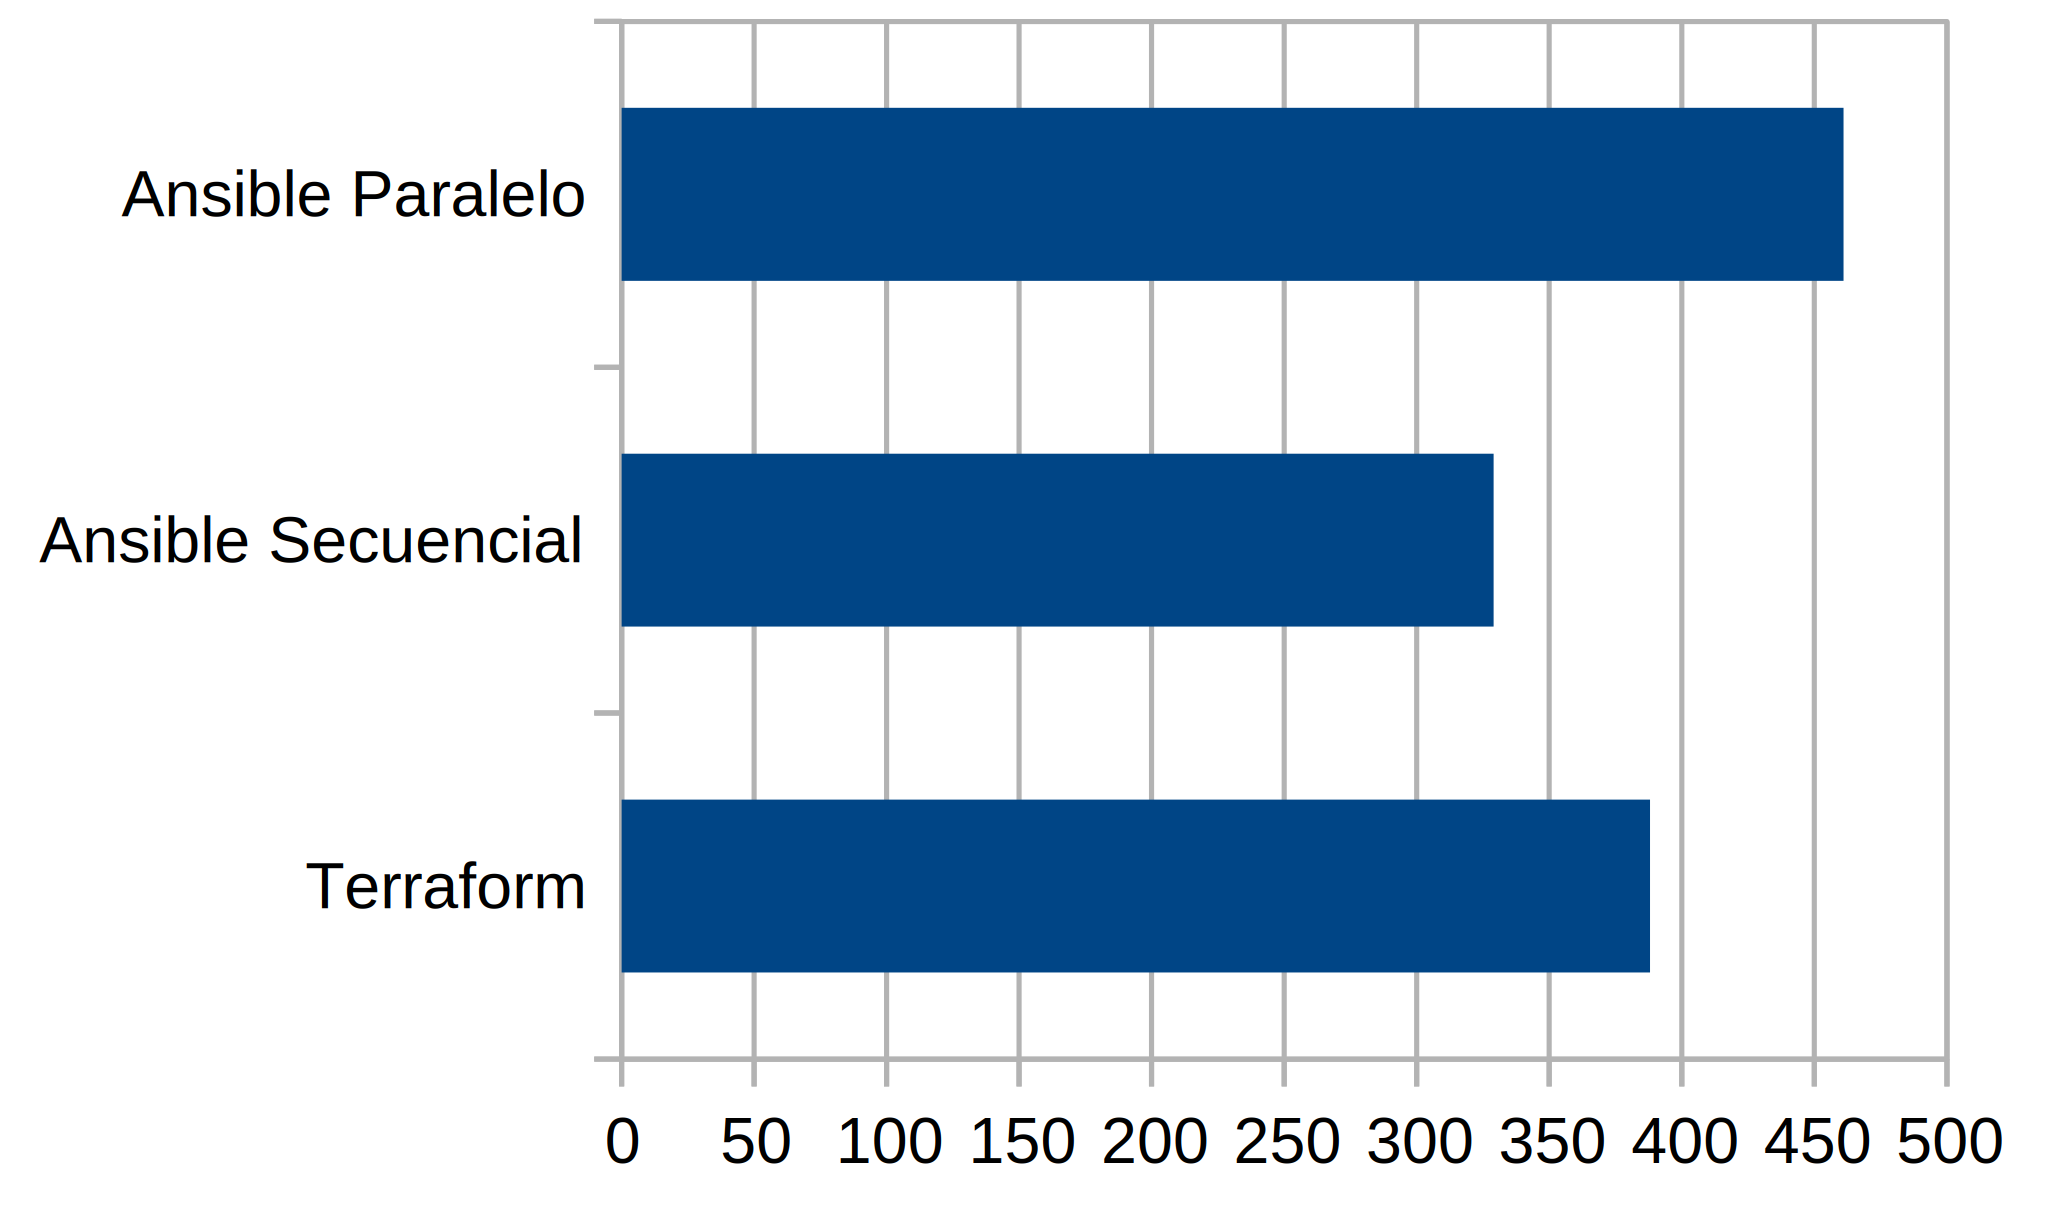
\includegraphics{../charts/lineas.pdf}
            }
            \caption{Líneas de código}
        \end{subfigure}
        \begin{subfigure}{0.45\textwidth}
            \resizebox{\linewidth}{!}{%
                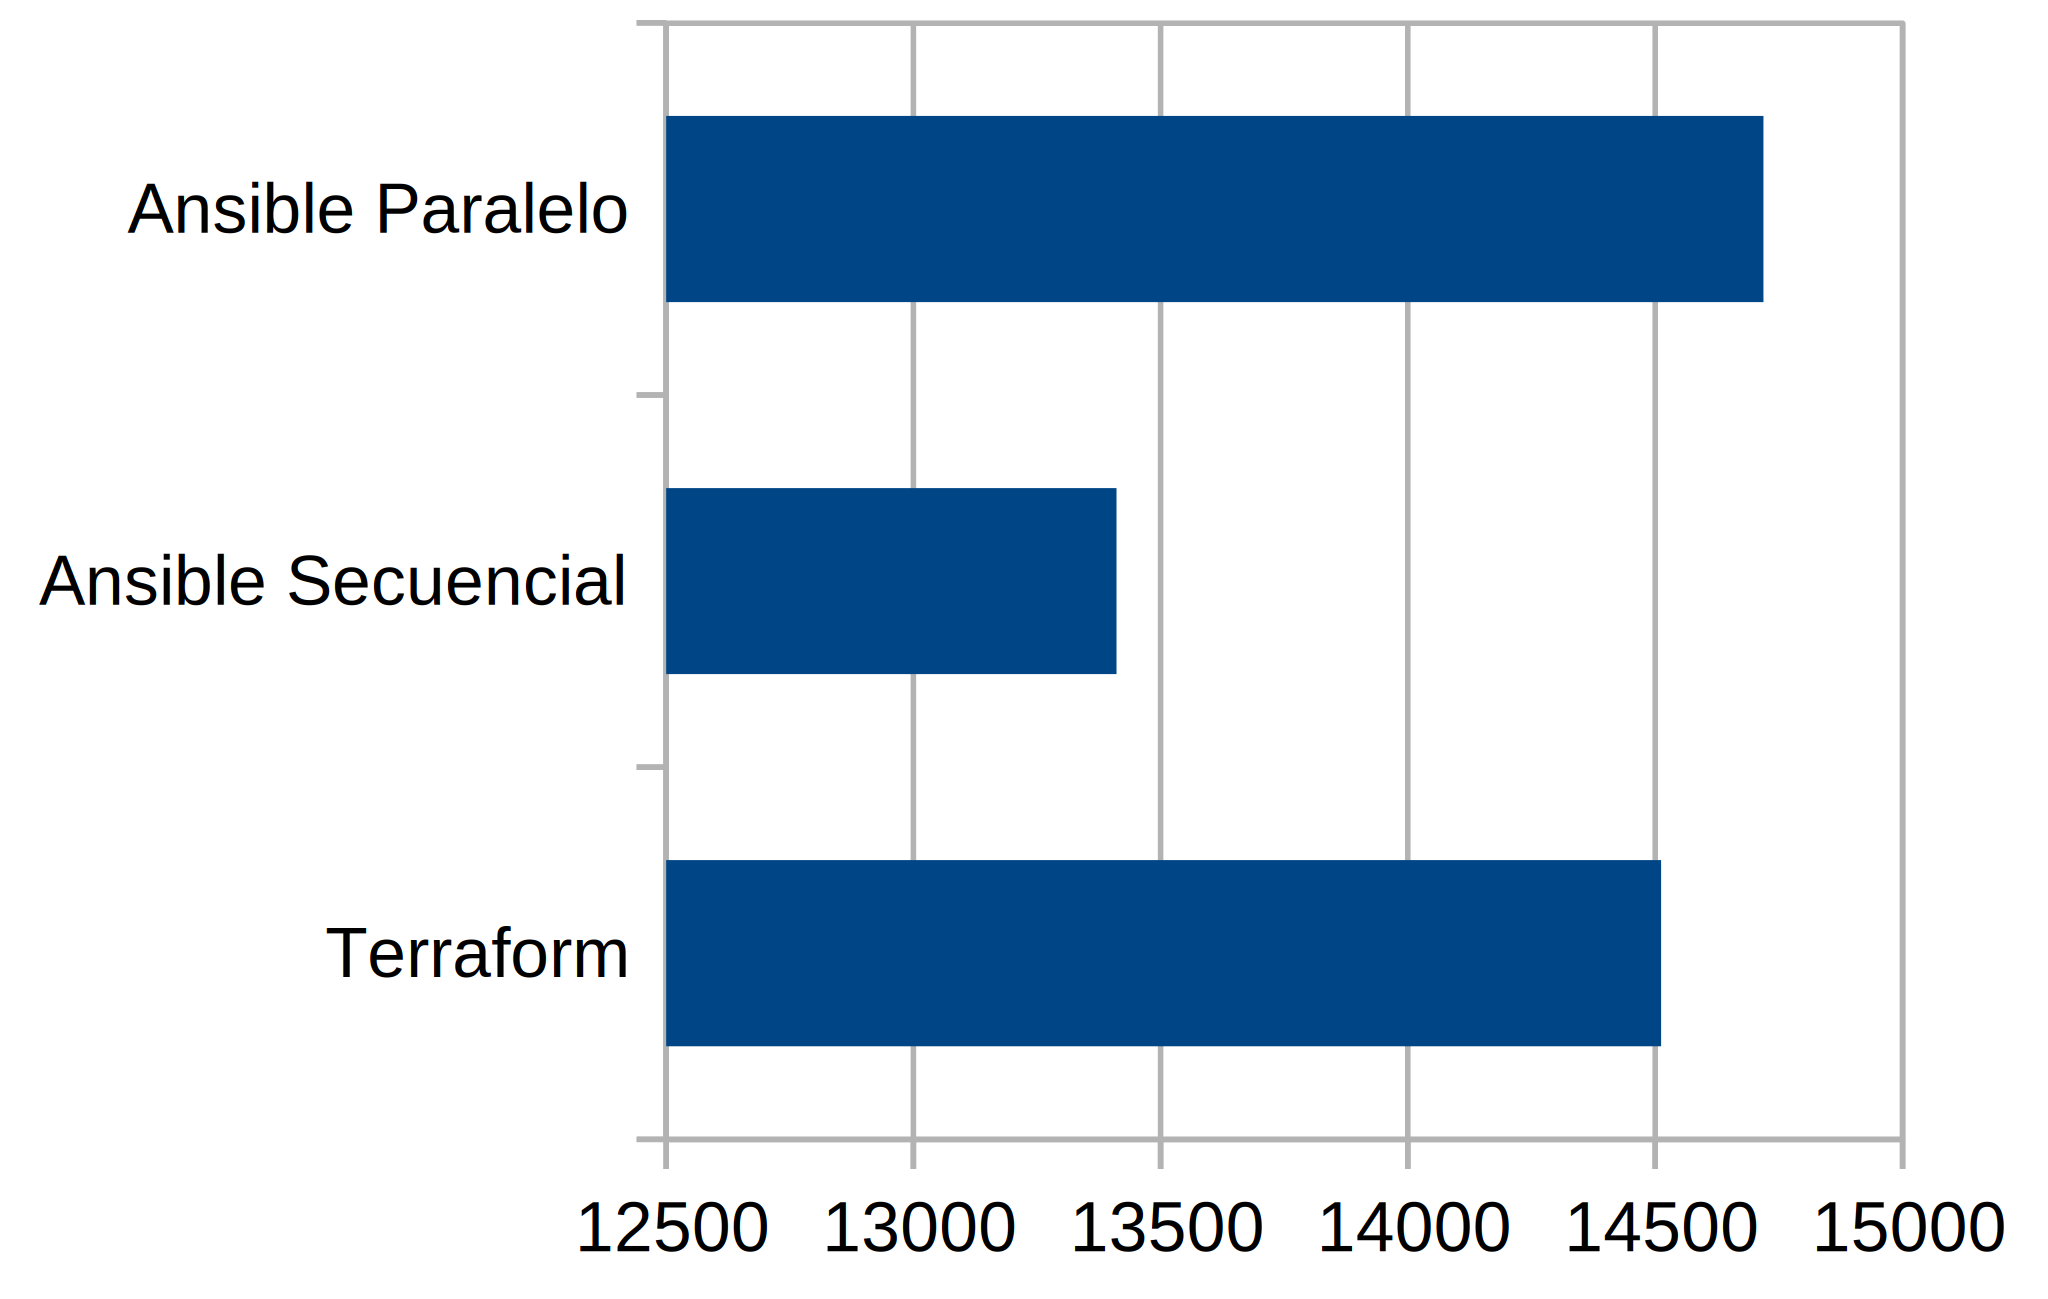
\includegraphics{../charts/caracteres.pdf}
            }
            \caption{Caracteres}
        \end{subfigure}
        \caption{Verbosidad de los proyectos (O. Salvador, 2023)}
    \end{figure} 


\clearpage
\subsection{Integración de una en la otra}
Estas herramientas no son mutuamente excluyentes. Como último ejercicio, me propuse implementar un playbook en el que se use el módulo de Terraform (\cite{terraform_ansible}) y mis proyectos de este para hacer el aprovisionado. Me apoyé sobre el siguiente artículo de Medium para aprender a usarlo y sus detalles: \cite{terraform_ansible_medium}. La implementación del playbook \texttt{terraform\_ansible} es muy sencilla, ya que solo se necesita una tarea para aplicar un proyecto, y el rol que la contiene pudiéndose reusar para los tres que tengo en Terraform.
\linebreak

\bigskip
        
        \begin{minipage}{.46\textwidth}
            Este playbook ha conseguido los mejores tiempos (Anexo \ref{anexo:tiempos}) para el despliegue de de la infraestructura base, mejores incluso que los de Terraform por su cuenta. Esto es sorprendente, ya que debería tener al menos ese tiempo, y encima el añadido del \textit{\gls{overhead}} de Ansible. Como posible explicación se me ocurrió que el módulo de Ansible reimplementase partes de Terraform, de manera más optimizada. Aprovechando que estos proyectos son abiertos, he revisado el código del módulo (\cite{terraform_ansible_module}). En el he descubierto que su implementación, en Python,
            \linebreak
            
        \end{minipage}% This must go next to `\end{minipage}`
        \hspace{1.5cm}
        \begin{minipage}{.41\textwidth}
            \inputminted[fontsize=\scriptsize, firstline=25, lastline=34, linenos, frame=single, breaklines]{yaml}{../../ansible/terraform_ansible/terraform/main.yml}
            \vspace{-.4cm}
            \captionof{figure}{Tarea de despliegue en\\\texttt{roles/terraform/task/main.yml}\\(O. Salvador, 2023)}
            \vspace{.4cm}
            
        \end{minipage}
        \vspace{-.25cm}
        
tiene sencillamente una función en la que lanza el comando CLI después de convertir los campos de la tarea a opciones de este. Sí que realiza un plan. Habiendo explorado esta posibilidad y sabiendo que había seguido el mismo método para todas las mediciones, la posibilidad más probable es que no controlase suficientes variables durante el estudio. Aunque hice cinco medidas, realicé las de este playbook días después de los otros, y Azure podría haber tenido menos demanda durante este.
\linebreak

La verbosidad de esta solución es solo ligeramente superior a la de Terraform suelto, ya que deja poco que implementar. El módulo de Terraform incluye \underline{todas} sus funcionalidades, incluida la actualización de recursos.
\linebreak

También hay módulos de Terraform para trabajar con Ansible (como \cite{terraform_ansible_cloud}), pero no son oficiales ni populares. Aparte, se puede conseguir ejecutando el comando \texttt{ansible-playbook} en un recurso aprovisionado (\cite{terraform_ansible_digitaloc}). Ninguna de estas opciones integra Ansible de manera comparable con la inversa. Por tanto, no las he perseguido.





\clearpage
\section{Conclusión}
Terraform es una mejor herramienta de aprovisionamiento. Es más fácil de hacer funcionar, aprender, rápido desplegando y de desarrollar para las funcionalidades que proporciona. Ansible no tiene, de serie, los lujos que ofrece su alternativa, e implementarlos incurre un coste. Para que un playbook compita con todo lo que trae Terraform, tendrá que ser más verboso y complicado de leer. Su alternativa envejecerá mejor, y podrá ser entendido por gente con menos experiencia.
\linebreak

Si en la empresa me pidiesen elegir una herramienta, recomendaría Ansible. Por supuesto, dependería del uso particular, y ofrecería contexto que he aprendido durante esta práctica. Sólo he sido testigo de Ansible usado en producción, y los playbooks que he visto podrían replicarse casi por completo en Terraform. Pero no en su totalidad. Esta pequeña cantidad de pasos que no se pueden conseguir sin integrarlo en otro sistema, al contrario que Ansible, son lo que le da al último su ventaja. Terraform tendrá que ser fuertemente acoplado a un pipeline o script en el que solo sea un paso, mientras que un playbook es el propio pipeline, englobando todos los pasos necesarios. Esto lo hace más portátil y agnóstico a la plataforma de CI/CD.
\linebreak

En la mayoría de casos, el tiempo que ahorra paralelizar un playbook no justifica hacerlo. Igualmente, los mejores tiempos de Terraform no triunfan sobre Ansible de la manera que sus módulos adicionales y funcionalidades (fuera del aprovisionamiento) añadidas lo hacen a la inversa. Cuanto mayor sea el proyecto, más se beneficiará de la abstracción, rendimiento y utilidades que da Terraform. Pero también se vuelve más probable que tenga necesidades que Terraform solo no es capaz de suplir. 
\linebreak

El bagaje del su origen sobrecomplica Ansible, pero ambas herramientas se pueden aprender en una semana. Conseguir el código básico para la infraestructura es más rápido en Ansible, y donde sea necesario, se puede profundizar para implementar las funcionalidades. Si aún así no es capaz de satisfacer el proyecto, se puede integrar Terraform, y conseguir todos sus beneficios, dentro de Ansible, mientras que no se podría de haber elegido Terraform primero.
\linebreak

En resumen, la flexibilidad de Ansible lo hace una mejor herramienta para navegar los requisitos de despliegue de una aplicación, sus necesidades y su infraestructura, mientras que Terraform es preferible para proyectos que no escapen de su ámbito.









\clearpage
\appendix
\section{Generación grafico del grafo de dependencias}
\label{anexo:grafico}
En su documentación, \cite{hashicorp_graph}, explica como imprimir el grafo de dependencias como texto, y usar \texttt{dot} para convertirlo a un gráfico. Como el diagrama que sale por defecto es muy plano, ya que el objetivo de Terraform es encontrar las dependencias y maximizar las operaciones que pueda paralelizar, el grafo es muy plano. A su comando, que solo usa \texttt{dot}, le he añadido otra herramienta, \texttt{unflatten}, que intenta hacer los grafos más verticales. Las opciones \texttt{-l} y \texttt{-f} del comando \texttt{unflatten} indican la cantidad de niveles o filas, y la reorganización de las flechas respectivamente. La opción \texttt{-Tpdf} de \texttt{dot} es el formato de salida, PDF.
\linebreak

    \begin{figure}[htb]
        \centering
        \footnotesize
        \texttt{terraform graph | unflatten -l 45 -f  | dot  -Tpdf  > base-graph.pdf} 
        \caption{Comando para generar diagramas de los grafos de Terraform (O. Salvador, 2022)}
    \end{figure}



\bigskip

\section{Tiempos de aprovisionado de las herramientas}
\label{anexo:tiempos}
Estos tiempos son la media de cinco ejecuciones por cada herramienta y escenario. He abreviado ``Aprovisionado'' y ``Docker''. ``Docker'' implica la construcción de la imagen, etiquetado, y subida al registro de Azure. En cada herramienta he construido las imágenes después de borrar todas las que tenía el sistema, para que empezaran desde cero. En el caso de Terraform, la construcción a la que se refiere es manual, haciéndola con los comandos que muestro en la Figura \ref{comandos_docker} (p. \pageref{comandos_docker}). Dicho esto, entre el frontend y backend no las he borrado, y se refleja en el frontend heredando capas y tardando menos. En un caso de uso real, no se borrarían las imágenes entre pasos. Terraform necesita generar un plan antes de aplicarlo, y he optado por generarlo antes de aplicarlo, en lugar de dejar a Terraform hacerlo durante el \texttt{apply}. De ahí que sus tiempos estén desglosados. Tardaría menos como un único paso, pero sería mala praxis. Los tiempos de Docker en Ansible Terraform son los mismos que en secuencial.
\linebreak

\setcounter{table}{0}
\begin{table}[h!]
    \centering
    \begin{tabular}{| l | r | r | r | r | r |}
        \hline
        \textbf{Herramienta} & \textbf{A. base} & \textbf{A. Backend}      & \textbf{A. Frontend}    & \textbf{D. backend} & \textbf{D. frontend} \\
        \hline
        \hline
        Terraform            & 15s + 20m 28s    & 17s + 1m 48s             & 16s + 1m 50s            & 1m 33s              & 3m 21s               \\
        \hline
        Ansible Secuencial   & 23m 31s          & 2m 23s                   & 1m 52s                  & 1m 41s              & 3m 42s               \\
        \hline
        Ansible Paralelo     & 19m 36s          & 1m 47s                   & 1m 50s                  & 1m 38s              & 3m 59s               \\
        \hline
        y docker paralelo    & -                & -                        & -                       & \multicolumn{2}{c|}{6m 14s}                \\
        \hline
        Ansible Terraform    & 19m 12s          & 2m 11s                   & 2m 13s                  & -                   & -                    \\
        \hline
    \end{tabular}
    \caption{Tiempos medios de aprovisionado}
    \label{tiempo_aprovisionar}
\end{table}






\clearpage
\section{Verbosidad de los proyectos y playbooks}
\label{anexo:verbosidad}

He conseguido estas cifras usando tres herramientas de CLI: \texttt{cloc}, \texttt{wc} y \texttt{find}. La primera cuenta las líneas de código, excluyendo comentarios y líneas en blanco. La segunda, con la opción ``\texttt{-c}'', cuenta el número de caracteres en un fichero. Con la tercera elijo los ficheros que alimentar a la anterior.
\linebreak

\begin{table}[h!]
    \centering
    \begin{tabular}{| l | l | r | r | r |}
        \hline
        \textbf{Fichero(s)}                 & \textbf{Métrica} & \textbf{base}   & \textbf{backend}  & \textbf{frontend}           \\
        \hline
        \hline
        
        \multirow{2}{*}{variables.tf}       & Líneas de código & 36              & 36                & 33                          \\
                                            & Caracteres       & 1324            & 1400              & 1007                        \\
        \hline
        \multirow{2}{*}{Resto}              & Líneas de código & 112             & 92                & 79                          \\
                                            & Caracteres       & 3906            & 3977              & 2898                        \\
        \hline
        \multirow{2}{*}{Total}              & Líneas de código & 148             & 128               & 112                         \\
                                            & Caracteres       & 5230            & 5377              & 3905                        \\
        \hline

    \end{tabular}
    \caption{Verbosidad de los proyectos de Terraform}
    \label{verbosidad_terraform}
\end{table}

\bigskip

En el playbook \texttt{parallel\_ansible} uso dos plays, que no he contado en el total. He contado la play serial, que tiene 21 líneas de código y 505 caracteres. La que usa la estrategia free tiene 46 y 745. Tampoco he incluido en ninguno el rol de Docker, al que Terraform no tiene equivalente. De la misma manera, excluyo de los resultados del rol ``destroy'' del playbook paralelo, ya que solo está ahí. Una tercera parte de las lineas y quinta de los caracteres de Terraform son los ficheros \texttt{variables.tfvars}
\linebreak

\begin{table}[h!]
    \centering
    \begin{tabular}{| l | r | r |}
        \hline
        \textbf{Herramienta/Playbook}     & \textbf{Líneas de código}  & \textbf{Caracteres} \\
        \hline
        \hline
        
        Terraform                         & 388                        & 14512               \\
        \hline
        Ansible Secuencial                & 329                        & 13411               \\
        \hline
        Ansible Paralelo                  & 461                        & 14719               \\
        \hline
        Terraform en Ansible              & 44+388                    & 3511+14512           \\
        \hline

    \end{tabular}
    \caption{Verbosidad de Terraform y Ansible}
    \label{verbosidad_todos}
\end{table}
















\end{flushleft}

\clearpage
\printbibliography[heading=bibintoc, title={Bibliografía}]

\end{document}
